% ------------------------------------------------------------------------
% A Latex template created by Dr. Wenjia Wang for CMP MSc Dissertation. 
% 
% Lasted update: 24/03/2020 by Wenjia Wang
%----------------------------------------------
% Please read the in-file brief Instructions below 
% or More detailed Instructions in sample file (Instructions.tex)
% to learn how to use this Latex template.
% 
% Then go through from current line number 155 to line 205
% to fill in the details about yourself, course, your dissertation, etc. 
%
% Notes and sample files:
% "acronyms.tex": a sample file where you define your abbreviations.
% ------------
% 
% ####---- Brief in-file Instructions ----####
% ----Preparation steps: 
% (i)  Download the zipped Latex template file into your disk or your university's home space on U disk,
% (ii) Unzip all the files into your working folder, such as \Dissertation. 
% (ii) Change/replace/fill some places in this "DissertationTemplateV.tex" file (where V is the version number, e.g. 5)  to suit your need:
% 	such as, Your course, year, dissertation title, your name, markers, etc.
%
%% Then you can follow the instructions (not necessarily in that order) to write your dissertation. 
%   
%% 1. Write your abstract in a provided sample tex file: "Abstract.tex"
%% 2. Write your acknowledgement in a provided sample tex file: "Acknowledgement.tex"  
%    Note: Both tex files are already included in the zipped file. 
%
%% 3. Write each chapter in a separate tex file and name them e.g. Ch1.tex, Ch2.tex, etc. 
% and then use "include" to include them as shown in this example.
% 
%% 4. Citation styles: package "natbib" is used for making references.
%   you should replace the bib file - xbib, with your own bib file
%   at the END of this template file, i.e.   
%   \bibliography{xbib} % use your own bib file 
%   Then, you can use the following two commands 
%   to cite your reference, pending on how it is use. 
%   (i) Use Command "\citep{...}" to produce the style: (Authors, year)
%   (ii) Use Command "\citet{...}" to produce the style: Authors (year)
%
%#### 
% If you wish to produce a list of abbreviations/acronyms 
% that are used in your dissertation, you must read notes 5-8 below. 
%
%% 5. Define abbreviations or acronyms
% 	you can use the given sample file "acronyms.tex" 
% 	to define your abbreviations or acronyms, and 
% 	some examples are already defined in that file.
% 	After you have defined them, (you can add any new items anytime you like), 
% 	save it in the same folder of your dissertation main tex file
% 	as it is included by using "include{acronyms}" in this file later.
% 	Note: if you use any other file name, change it in "\inlcude{yourFilename}. 
%
%% 6. Using the defined abbreviations/acronyms
%   In file "IntrsuctionsV.tex", I explain and show how to use defined acronyms in your tex file.  
%
%% 7. Generate a List of Abbreviations(LOA)
%  You must issue command "Makeglossaries" to produce few more auxiliary files 
%   e.g. xxxx.acr, and/or .glo, and/or .gls, etc. in order to produce LOA 
%   so, is you use TexStudio, Click "Tools" and choose "Makeglossaries"
%
%% 8. Don't want to have a list of Abbreviations
%  use command "\nolistofabbs", by uncomment it in later part  
%  then LOA will not be generated and not appear in the TOC. 
%  note: you may have to run "Build and View" twice to get the intended result.
%        first run to remove/get the acutal list of abbreviation
%		 second run to remove/get the list appearing on TOC.   
% 
%% 9. Using footnote. (% wjw, added this note on 11/09/2015)
%	If you want to use footnotes in any chapters of your dissertation, 
%	you can use command \footnote{your footnote text} in where you want.
% 	The footnotes are numbered automatically and continuously within a CHAPTER.   
%   
% 10. Added the confidentiality statement on 24/03/2020. 
%
% 
% Disclaimer: This template is provided as it is. 
%  You should not change it if you are not sure what you are doing.  
%  Dr. Wang won't be held responsible for any problems it has or causes,
%  although you should let me know if you found any bug.
%
% ------------------------------------------------------------------------
\documentclass[a4paper, 12pt]{report}
\usepackage[centertags]{amsmath}
\usepackage{amsfonts}
\usepackage{amssymb}
\usepackage{amsthm}
\usepackage{newlfont}
\usepackage{graphicx}
\usepackage{natbib} % by wjw 22/11/2016 to replace apalike package
%\usepackage{pdfsync} %PDF Forward Search
\usepackage{color}
\usepackage{enumitem}
\usepackage{float}
\usepackage[acronym]{glossaries} % added by wjw on 05/08/15
\usepackage{datetime}

\usepackage{CMPDissertation5} % CMP Dissertation Style

\usepackage{XTocinc} % Include Table of Contents as the first entry in TOC

\usepackage{setspace}  % added by wj on 11/09/15
% Note: this makes the body text in chapters are double spaced 
% and text in table are single spaced.
% If you want to have a double space in tables, commented it out. 

%\usepackage[active]{srcltx}  %SRC Specials for DVI search

% Fuzz -------------------------------------------------------------------
\hfuzz2pt % Don't bother to report over-full boxes if over-edge is < 2pt
% Line spacing -----------------------------------------------------------
\newlength{\defbaselineskip}
\setlength{\defbaselineskip}{\baselineskip}
\newcommand{\setlinespacing}[1]%
           {\setlength{\baselineskip}{#1 \defbaselineskip}}
% As the package setspace is included above, which define linespacing, 
% the following newcommands for double/single spacing become redundant, 
% hence they were commentted out. wj 11/09/2015   
%\newcommand{\doublespacing}{\setlength{\baselineskip}{2.0 \defbaselineskip}}
%\newcommand{\singlespacing}{\setlength{\baselineskip}{\defbaselineskip}}

%
\numberwithin{equation}{section}
\renewcommand{\theequation}{\thesection.\arabic{equation}}

%%% ----------------------------------------------------------------------
\setlength{\tclineskip}{1.05\baselineskip}
%%% ----------------------------------------------------------------------
%\nobib
%\draft
%\nofront
%\permissionfalse

%\dedicate{}

\nolistoftables
\nolistoffigures
% if you don't want to have a list of Abbreviations
% uncomment the following command
\nolistofabbs

% This is an MSc dissertation
\msc

% if this is for  PhD thesis
%\phd

\university{The University of East Anglia}
\school{Computing Sciences}

%%%%%% You need to change/fill few things from here %%%%%%

%#### CHOOSE OR INSERT YOUR MSC COURSE TITLE BELOW #####
% by commentting in your course from the list below.

%\course{Advanced Computing Science}
\course{Computing Science}
%\course{Cyber Security}
%\course{Data Science}


%####---- change the year and month to fit your course dates ####
%\monthyeardate\today

\copyrightyear{2024}   % change to your submission year.
\submitdate{August, 2024} % Change to your submission date: month, year.
%\submitdate{\date{today}}
\studyyears{2023}{2024} % change to your start and finish years of your course.
%\convocation{July}{2022}

%####---- SET CONFIDENTIALITY RESTRICTION ----------
%### uncomment the following two lines if your dissertation is confidential

%\confidential{}   	% display the confidentiality statement on the title page  
%\setconfidentialdate2{August 31, 2023} %% set the end date to e.g. August 31, 2023

%% it will the produce a statement on the title as follows:
%% --- CONFIDENTIALITY STATEMENT:
%% The contents of this dissertation remain confidential until August 31, 2021
%% and should not be discussed or disclosed to any third party without the prior written permission 
%% from the School of Computing Sciences, the University of East Anglia.

%%--------------------------------------------


% ---------------------------------------------
% #### Insert the title of your dissertation below.#####
\title{Comparing Single-task Learning and Multi-task Learning in Mental Health Prediction in Schizophrenia Patients}

% #### Insert your full name below.#####
\author{Olajumoke Ore Akinremi}

%#### insert your supervisor's name below #####
\supervisor{Dr. Min Aung}

%#### insert the name of your markers if you know them #####
%#### Markers are usually allocated in July #### 
\firstmarker{Marker 1: Dr. Min Aung} % your supervisor usually 
\secondmarker{Marker 2: Dr. Cheng Wang}

%#### leave the following two lines as they are ####
\examiner{Checker/Moderator}
\organiser{Dr. Wenjia Wang}

%#### include a tex file here, e.g. acronyms.tex, 
%#### where you have defined your acronyms and abbreviations.   
%####
% File name: acronyms.tex
% purpose: a sample file that is used to define abbreviations, acronyms, glossary.
% Created on 05/08/2015, by Wenjia Wang

%#### Notes:
% In this file, you can define all the abbreviations you wish to use in your text.

% 1. Use command "\newacronym" to define an abbreviation/acronym 
% format: \newacronym{label}{name}{description}
% for example:  

\newacronym{mtl}{MTL}{Multi-task Learning}
\newacronym{stl}{STL}{Single-Task-Learning}
\newacronym{ema}{EMA}{Ecological Momentary Assessment}
\newacronym{lassoCV}{LassoCV}{Least Absolute Shrinkage and Selection Operator model}

% 2. use command "\gls{label}" or "\Gls{label}" to cite a defined acronym in your .tex file 
% for example: \gls{UEA}
% when used it in the first time, it will produce: University of East Anglia(UEA)
% when used after the 1st time, it will produce: UEA    

% Some more examples defined here.

\newacronym{api}{API}{Application Programming Interface}
\newacronym{uml}{UML}{Unified Modelling Language}
\newacronym{kdd}{KDD}{Knowledge Discovery form Database}
\newacronym{svm}{SVM}{Support Vector Machine}


% or use the following command to define a glossary term %"\newglossaryentry{label}{name={<name>}, description={<describing blahh blah}}
% e.g

\newglossaryentry{apple}
{
	name={apple}, 
	description={is a kind of sweet fruit}
}
\newglossaryentry{latex}
{
	name=Latex,
	description={is a mark-up text-editing language specially   
		for writing scientific documents}
}

\makeglossaries

%------------------------------------------------------------------------
\begin{document}
{
\typeout{:?000000000} % Don't bother with over/under-full boxes
\beforepreface
\typeout{:?111111111} % Process All Errors from Here on
}

\afterpreface
\def\baselinestretch{1}
\setlinespacing{1.66}

%--------------------------------------------------------------------

%------------------------------------------------------------------------

% ##### Include each chapter in order below #####
%% Notes for using the Latex Dissertation Template, created by Wenjia Wang. 
% wenjia.wang@uea.ac.uk
% ------------------------------------------------------------------
\def\baselinestretch{1}

\chapter{How to Latex}

\def\baselinestretch{1.66}

%%% ----------------------------------------------------------------------
This LATEX template was created by Dr. Wenjia Wang\footnote{Created in 2005 based on CMP thesis style file and one from Stanford University. 

Previous versions: created in 2005 (v0), updated in 2010(v1) and 2012(v1.1).  
	Major Revision on 06/08/2015-17/08/2015(v2): Added the function of generating the list of Abbreviations (you must follow the instructions carefully and exactly in order to produce a list of Abbreviations). 
	Major revision on 22/11/2016(v3), added notes for how to use the Template.   
	Updated on 15/04/2019: Updated the Instruction .
	
	updated on 24/03/2020(v4) and August 2021(v5): revised latex style file to typeset the dissertation title page in bold, as per the dissertation handbook, and added a confidentiality statement. 
	Tidied up some small issues in Instructions and Citations, e.g. changed ``Bibliography" to ``References" at the very end.
	And also gave an example for creating an entry for citing a web source in bib file, with URL and the accessed date. 
}
 to be used by the Master students at the \gls{cmp}, the \gls{uea}, to write their dissertation with Latex. 

This section gives you the sufficient instructions on how to use the template so you must read it carefully before using it.

NOTE: you should use $TexStudio$ as your text editor and Latex compiler to make sure this Latex Template working properly, although it may work with other text editors.

If you use Overleaf, you should create a project on it and name it, e.g. ''Dissertation". Then you need to upload ALL the files contained in the zip files. 

Choose the main tex file -       
 
Please let me know if you find any bugs or problems, although I may not have time to resolve them in time.
 
 
\section{How to use this Latex Template}
 
\subsection{Preparation Steps: P1 to P4} 
 
P1. Download the template package from the blackboard of Dissertation Module and Unzipped it to an intended working folder on your U (University) drive, or any other drive on your Computer, e.g. Dissertation. 

Note, you are strongly recommended to use the University's file storage on U drive as your main working folder because you can access it from any PCs on Campus and also your own PC via VPN. In addition, you must have a backup storage to save all your working files and programs developed for your dissertation.     

P2. Start TexStudio and open ``DissertationTemplate5.tex"

and before doing anything, save it to another tex file, e.g. named "Dissertation.tex", as your own dissertation MAIN file. 

Note: This main Latex file  

(i) uses, i.e. includes all the other files, such as Abstract, Acknowledgement, and all your Chapter tex files, Appendix etc., which are written separately with Latex.
 
(ii) generates a pdf file of your dissertation as a whole.         
 
P3. You MUST change/replace/fill a few places in this file, i.e. your main tex file, to suit your need. 
More Specifically, you need to go to LINE 155 and do 

(1) Choose/Comment in your course from the given list;

(2) Change the year of your study, 

(3) Decide the confidentiality: if your dissertation is Confidential,  comment in the 2 command lines as indicated and change the year of restriction;

(4) Fill in your Dissertation Title, your name, markers, etc.

\textcolor{red}
{Note: If your dissertation is considered to be confidential}, you and your supervisor need to decide an end date (month day, year) of confidentiality. Then you need to UNCOMMENT the two lines in the template file, where are indicated in the template tex file, which copied over here to show what they look like. 

 $\backslash confidential\{\}$   	\% display the confidentiality statement on the title page  
 
 $\backslash setconfidentialdate2\{August 31, 2021\} $	\% set the end date to e.g. August 31, 5

Once they are uncommented, and a specific date, e.g. August 31, 2021, is set, the pre-written confidentiality statement and the end date will be displayed in red colour on the title page, as shown below.
  
\textcolor {red} {	
	{\emph{CONFIDENTIALITY STATEMENT:\\ 
		The contents of this dissertation remain confidential until \underline{August 31, 2025}
		and should not be discussed or disclosed to any third party without the prior written permission 
		from the School of Computing Sciences, the University of East Anglia.}}}


P4. If you have not saved your tex file to a new file yet, save it with a new file name to a folder specially created for writing your dissertation, e.g. ``Wang\_Dissertation2020.tex" 


\subsection{Work on each latex file}
		
Then following the steps below to work on each file to write your dissertation.    

 1. Write your abstract in a separate tex file and name it as \emph{Abstract.tex}
 
 2. Write your acknowledgement in a separate tex file and name it as \emph{Acknowledgement.tex}
   
 Note: Both \emph{Abstract.tex} and \emph{Acknowledgement.tex} files are already included in the style file.
 So you must not change their names but only the contents.    

 3. Write each chapter in a separate tex file and name them as, e.g. Ch1.tex, Ch2.tex, etc. 
 and then use ``$\backslash$include\{...\}" to include them as shown in this example.
 
(New notes added on 06/08/2015)

4. If you wish to produce a list of Abbreviations/Acronyms 
 that are used in your dissertation, you must read the notes given in Section \ref{Sec_Abbr}. 
%
% (4.1) Define abbreviations or acronyms
% 
% 	You can use the given sample file ``acronyms.tex" 
% 	to define your abbreviations or acronyms, and 
% 	some examples are already defined in that file.
% 	After you have defined them, (you can add any new items anytime you like), 
% 	save it in the same folder as this template file,
% 	as it will be included by using "include{acronyms}" in this file later.
% 	Note: if you use any other file name, change it in ``inlcude{yourFilename}". 
%
% (4.2) Use the defined abbreviations/acronyms
% 
%   In file ``acronymNotes.tex", I give some notes and few examples 
%   to explain and show how to use defined acronyms in your tex file.  
%
% (4.3) Generate a List of Abbreviations(LOA)
% 
%  You must issue command ``Makeglossaries" to produce few more auxiliary files 
%   e.g. xxxx.acr, and/or .glo, and/or .gls, etc. in order to produce LOA 
%   so, is you use TexStudio, Click ``Tools" and choose ``Makeglossaries"
%
%  (4.4.) Don't want to have a list of Abbreviations
% 
% Use command $\backslash$nolistofabbs, by uncomment it in later part  
%  then LOA will not be generated and not appear in the TOC. 
%  note: you may have to run ``Build and View" twice to get the intended result.
%        first run to remove/get the actual list of abbreviation
%		 second run to remove/get the list appearing on TOC.   


5. Using footnote (Wenjia added this on 11/09/2015)
 
 If you have to use footnotes (although you should try to avoid using any) in any chapter of your dissertation, 
you can use command $\backslash$foodnote\{foodnote text\} in where you want, for example, a footnote is included here.\footnote{Your footnote text: If you want to generate a list of Abbreviations, you must follow the instructions given here carefully and exactly, particularly using Command ``Makeglossaries" in ``Tools" before Compiling.} 
	
The footnotes will be automatically numbered continuously within a CHAPTER. 

6. Added the confidentiality statement and the end date, as described above (24/03/2020).  


\section {Making Citations and Citation Styles}

You are required to use the Harvard style for citing references in your dissertation.

Specifically, there are two sub-styles to be used in different situations, when using package ``natbib", which is included at the preamble of the template file.

1. Use command $\backslash citep\{...\}$. 

If the authors of a reference are NOT part of your sentence, e.g. ``A study (Wang, 2008) has been done to investigate the influence of some factors on the accuracy of an ensemble.", then use $\backslash$citep\{...\} in your Latex file, such as ``A study $\backslash$citep\{Wang08\} has been done...", it then produces the text as: 
``A study \citep{Wang08} has been done......"

2. Use command $\backslash citet\{...\}$.

If the authors of a reference are part of your sentence, e.g. ``Wang (2008) studied the factors that can affect the performance of a machine learning ensemble.", then use $\backslash$citet\{Wang08\} studied ... . It then produces the text as: `` \citet{Wang08} studied ......" 

3. Cite a web source

If you find a source from a web site and you want to include its URL and the accessed date in your reference list, firstly, you can create an entry in your bib file by using the entry style  `@misc\{ \}". See an example entry in the given bib file.

%misc{Wang_TrainDelayPrediction,
%	Author = {Wang, Wenjia and Parr, Gerard},
%	title = {Intelligence Ensemble System for Predicting and Preventing Train Delays},
%	year = {2019},
%    url = {https://www.uea.ac.uk/web/groups-and-centres/train-delay-prediction},
%	note = {Accessed on 24/08/2020}
%}

Then you can any of the citation commands as described above. E.g.\citet{Wang_TrainDelayPrediction}, leading a team from UEA and Greater Anglia, won a grant prize at the RSSB big data sandbox competition to carry on a research on developing machine learning ensemble methods for predicting train delays. 

4. To compile all your citations

Before building your complete Latex file,  
in TeXStudio, you should compile your bibliography first. You can press function key ``F8"  to do it, i.e. to pull all the cited references out from your Bib file and generate a bbl file. Check the message to see if there is any error in this process.

If you found that there is no change to your references, you should clean all your auxiliary files first and then repeat the above procedure


\section{Creating Equations}

You can write an equation, as shown in Equation \ref{Equ_simLinear}, by using $\backslash$begin\{equation\} write equation here $\backslash$ end\{equation\}. For example, 

\begin{equation}
\label{Equ_simLinear}
y = a + b_1x_1 + b_2x_2
\end{equation}

If your equation is too long for a single line, instead of using the above environment,  
use ``$\backslash$begin\{align\}" command to align an equation of multiple lines at a specified point. 
Use $\backslash\backslash$ to specify a line break, and \& to indicate where  the lines should be aligned. 

For example, the following equation, as shown in Equation \ref{Equ_quardrFunc}, is aligned at ``=". 

\begin{align}
\label{Equ_quardrFunc}
f(x) &= (x+a)(x+b) \nonumber \\
&= x^2 + (a+b)x + ab
\end{align}

Equation \ref{Equ_complexFunc} is aligned at the left brace.  

\begin{align}
\label{Equ_complexFunc}
f(x) &= \pi \left\{ a + b_1x_1 + b_2x_2+ b_3x_3^4 + b_4{x_4}^3 + b_5x_5^2 \right.\nonumber\\
&\qquad \left. {} + b_6x_6^5 + b_7x_7^2+ b_8x_8^3 + b_9{x_9}^3 \right\}
\end{align}  

Note: ``\emph{\{align\}}" must not be nested within ``\emph{\{equation\}}", it replaces ``\emph{\{equation\}}".

If you do not want to automatically number an equation, use  \{equation*\} or  \{align*\}. For example, the following equation will not be numbered.   

\begin{equation*}
y = a + b_1x_1 + b_2x_2^2 + b_3x_3^3
\end{equation*}

\section{Define and generate a List of Abbreviations(LoA)}
\label{Sec_Abbr}

This section tells you how to define Abbreviations, generate a list of them and show the list on the preamble of your dissertation.
   
% text for testing abbreviations
I will show you how to use the acronyms defined in a given file named as ``acronyms.tex", which will be then listed in the \gls{loa} if THEY ARE USED in your Dissertation.

\subsection{Define abbreviations/acronyms}

( Notes and sample files:

``acronymNotes.tex": brief introduction on how to make a LoA. 
 
 ``acronyms.tex": a sample file where you define abbreviations.
)

To define an abbreviation or acronym, open the provided sample file in the template package - ``acronym.tex",  in any text editor, e.g. TeXStudio, you can see some abbreviations (or acronyms) already defined in it.

You can simply use the following command \emph{newacronym} to define an abbreviation/acronym 
in the format: $\backslash$newacronym\{label\}\{name\}\{description\}

For example:  
% the acutal command: \newacronym{uk}{UK}{The United Kingdoms} 
% but to show it in the complied text, 
$\backslash$newacronym\{api\}\{API\}\{Application Programming Interface\}\} 
 
\subsection{Use the defined Abbreviations/Acronyms}


You can use $\backslash$gls, or  $\backslash$Gls, Capital, to insert the abbreviation to anywhere you want in your tex file. 
Or use $\backslash$glspl, or  $\backslash$Glspl for using their plural forms. 

In the first time you use it, it will produce the full text of the abbreviation, followed by its abbreviation in (). After that, it will only produce the abbreviation.   

For example,      
$\backslash$Gls\{api\} 
%\Gls{api}
 will be shown as \gls{api}, i.e. 'Application Programming Interface (API)' 
(without the quotation marks), 
and will add a linked page number to where it is used, e.g. `1' in this case, and will be shown in the \gls{loa}. 

After that, $\backslash$Gls\{api\} will produce only the abbreviation, i.e. \gls{api}.

\gls{uml}, \gls{svm}, \gls{kdd} are some other abbreviation examples I defined in ``acrynom.tex" file. Their plural format can be produced by using command: $\backslash$glspl\{\}.
 e.g.  $\backslash$glspl\{uml\}, $\backslash$glspl\{svm\},  $\backslash$glspl\{kdd\}, which produce:   
% the acutal commands are as follows: 
    \glspl{uml}, \glspl{svm}, \glspl{kdd}.  

\subsection{Compiling your main tex file with an Abbreviation file}

If you have defined your abbreviations or acronyms in file ``acronyms.tex", and use some of them in your text file of other Chapters, such as in this note file, by using the commands given above, you must compile and build your integrating tex file (e.g. DissertationSample.tex) to produce the intended files, e.g. pdf file, with the steps given in the next Section in TeXstudio. 

Please note:

(1) Only the used acronyms will appear in the List of Abbreviations.

(2) notice the difference in using ``gls{}" and ``glspl{}"


\section{Compiling/Building your tex file}

After you have written each of your tex files for your chapters, you need to include each of them in your dissertation main latex file, using a command ``$\backslash$include\{...\}",  as shown in this example. 

Then, you compile your main latex file by following the steps below to produce the intended results, i.e. a PDF file of your dissertation with every thing included.   
  
1. Run ``Compile" or ``Build/View" by clicking their icon, or simply press the shortcut key F5.
(note: you may see a pdf file with your text, but it won't have the list of abbreviations.)

2. Run ``Glossary" or ``Makeglossaries": 

If you have a list of abbreviations defined in the file ``acronyms.tex", you must do this, otherwise the list won't be included in your dissertation.
  
Click ``Tools" and then choose ``Glossary" or simply press shortcut key F9. 

(If it is not working, you can try: Click ``Tools", and 
``Commands", and choose ``Makeglossaries" to run it.) 

Ignore any warning message.

Note: whenever you make any new entry to your ``acronym.tex" file, and/or use any abbreviation/acronym in your other tex file, you must do this step to update your generated ``.gls" file.   

3. Run ``Build and View" (or press F5) again. 
This time the pdf file should contain the actual list of abbreviations after the list of Figures and the title appears in the Table of Content(TOC).
          


%%%-----------------

%\def\baselinestretch{1.66}
%\medskip

%%% ----------------------------------------------------------------------
 % you can edit this out in your file, but keep the tex and pdf files 
% ------------------------------------------------------------------------
% -*-TeX-*- -*-Hard-*- Smart Wrapping
% ------------------------------------------------------------------------
\def\baselinestretch{1}

\chapter{Introduction}

\def\baselinestretch{1.44}

%%% ----------------------------------------------------------------------

This chapter introduces my dissertation topic: Comparing single-task learning (STL) and multi-task learning (MTL) models in predicting mental health symptoms in schizophrenia patients. It outlines the theoretical background, research motivations, and clearly defines the aim and objectives, forming the foundation for the technical analysis.

\smallskip

%%% ----------------------------------------------------------------------
\goodbreak
\section{Background}
Emil Kraepelin initially identified schizophrenia in the early 1900s. Emil labeled the condition as "dementia praecox," describing it as a gradually worsening mental illness with an unclear biological cause that typically starts during adolescence and results in significant and frequently permanent declines in cognitive and functional abilities ~ \citep{mcglashan1996early}~. Schizophrenia ranks among the 15 leading causes of disability globally ~\citep{james2020global}. Serious mental illnesses like schizophrenia, schizoaffective disorder, and severe bipolar disorder often involve psychosis, necessitating extended inpatient care and medical treatment. 

Psychosis disrupts clear thinking and reality perception due to delusional behavior, impacting a person's emotion, perception, behavior, and cognition \citep{wang2020predicting}. Schizophrenia affects fewer than 1\% of the general population, however, this figure rises to 10\% among people who have relatives who were diagnosed with the illness, such as parents or siblings. The majority of those with schizophrenia are not aggressive or violent but the risk of violence increases when the mental illness is not treated. In his study, \citet{Rasool2018SchizophreniaAO} revealed that genetic factors, environmental influences, and changes in brain structure are some of the leading factors causing Schizophrenia.

Developing nations are likely to experience slightly higher remission rates for schizophrenia, this may be due to simpler environmental conditions or stronger social support systems. The disorder often appears in early adulthood or late teens. People born in urban areas show a slightly higher prevalence of schizophrenia. For males, the peak onset age is between 15 and 25 years, while for females, it is delayed by about 3 to 5 years in females, leading to an equal prevalence among genders ~\citep{pearlson2000neurobiology}. However, a recent evaluation of data from 33 nations indicated that the prevalence of schizophrenia varies by geographic region ~\citep{Rasool2018SchizophreniaAO}. It impacts thinking, emotions, and behavior, often causing individuals to lose touch with reality and hear voices others do not. According to ~\citet{pearlson2000neurobiology}, in the United States, the yearly net medical expenses of schizophrenia have been projected to be \$37.7 \text{ billion}, with an indirect cost of \$117.3\text{billion}~ \citep{adler2020predicting}. This mental disorder is costly due to its early onset, chronic nature, and disabling effects, despite not being fatal. Symptoms fall into three categories: cognitive, negative, and positive, hallucinations and incoherent speech are examples of positive symptoms; decreased expressiveness and social disengagement are examples of negative symptoms. Worsening symptoms can lead to psychotic relapses, severely affecting personal relationships and employment. Early detection of relapse is crucial for timely intervention \citep{adler2020predicting}, whereas current clinical practices by clinicians are ineffective at early detection of behavioral precursors of schizophrenia. They are not scalable and fail to capture dynamic behavioral changes, resulting in interventions occurring at late stages of the disease like conventional face-to-face assessments \citep{canas2023counterfactual}. Brief Psychiatric Rating Scale (BPRS) used by clinicians to track symptoms of schizophrenia during routine clinical and conventional in-person evaluations usually take place every few months. However, between the visits, psychotic relapses might happen, significantly impacting the patient’s daily functioning and potentially endangering both the patient and their relatives. Developing tools to track symptom variations and detect early indicators of change is essential for assisting clinicians in making well-informed treatment decisions~ \citep{tseng2020using}. A computerized system that evaluates symptoms by modeling patient behavior might be valuable in predicting potential relapses, as shifts in behavior have been linked to the beginning of relapses~ \citep{zhou2022psychotic}. Smartphones and other mobile devices are being employed to gather data on users' behavior and physiological states to forecast mental health conditions \citep{tseng2020using}. At the same time, Machine learning (ML) has become a valuable tool, providing more objective and accurate detection methods \citep{thieme2020machine}. It has demonstrated numerous advantages in areas such as research, diagnosis, support, treatment, and clinical administration \citep{shatte2019machine}.  

One prominent example is the CrossCheck system, a sophisticated smartphone app developed for passive tracking and monitoring of symptoms related to schizophrenia \citep{adler2020predicting}. The CrossCheck study carried out at Zucker Hillside Hospital in New York City, monitored 150 outpatients diagnosed with schizophrenia over 12 months. The participants were assigned to two groups at random.: one group of 75 participants was assigned to use the CrossCheck smartphone, while the other 75 participants followed the usual treatment regimen. The study's objective was to forecast relapses, identified by clinical assessors, particularly focusing on the likelihood of a participant relapsing the following day.
The CrossCheck app utilized the Android activity API to determine if users were walking, stationary, cycling, tilting, or engaged in an unidentified activity. The app monitored conversation events (but not the content) and recorded daily sleep and wake times every 10 seconds during movement and 30 seconds when stationary. In addition, the GPS data was extracted and converted to track distinct locations and travel distances. The metadata on calls, texts, and phone unlocks were recorded and the ambient noise and light levels were also measured. The 10 Ecological Momentary Assessments (EMAs) questions were delivered via the Crosscheck app to the participants every Monday, Wednesday, and Friday to monitor schizophrenia symptoms. These symptoms included feelings of depression, stress, auditory hallucinations, visual hallucinations, fear of harm, calmness, sociability, sleep quality, mental clarity, and hopefulness. Responses were recorded on a scale from 0 (no symptom) to 3 (severe symptom) \citep{wang2016crosscheck}.  By integrating the passive sensing data with self-reported EMA,the researchers were able to predict the (EMAs) of participants. \citep{adler2020predicting} and \citep{wang2016crosscheck}. Previous studies utilizing the CrossCheck dataset revealed a significant relationship between variables such as sleep patterns, phone usage, mobility, conversations and self-reported schizophrenia symptoms. In his 2020 study, \citet{tseng2020using} demonstrated that the performance of multi-task learning (MTL) surpasses that of single-task learning STL when various algorithms are employed. This approach ensures that the model undergoes a balanced training process across both learning paradigms, allowing for a more robust comparison of their respective performances. Each symptom such as feelings of calmness, hope, sleeping, social, thinking and negative tasks such as feeling depressed, harm, seeing -things, hearing voices, and feeling stressed is trained independently in STL, whereas in MTL, several related tasks such as feeling calm, hopeful, sleeping, thinking are trained concurrently to improve generalization. For example, learning to predict feelings of calmness might also help improve the model's performance in predicting social engagement, as these tasks could share underlying psychological processes. This shared learning can result in better generalization of new, unseen data, leading to more reliable predictions in real-world scenarios. STL models, by focusing on isolated tasks, might overfit and fail to generalize well across different tasks. In complex mental health conditions like Schizophrenia, multi-task learning can capture the multifaceted nature of the disorder, potentially leading to more robust diagnostic tools and may offer a more comprehensive and accurate diagnostic solution offering insights that a series of independent STL models might overlook \citep{thieme2020machine}. 

This study builds on foundational research by advancing the analytical framework through the implementation of the Least Absolute Shrinkage and Selection Operator with Cross-Validation (LassoCV). LassoCV is adept at handling both Single Task Learning (STL) and Multi-Task Learning (MTL), through its MultiTaskLassoCV variant. The algorithm excels in feature selection and model regularization by shrinking less significant feature coefficients to zero, thereby enhancing model interpretability and robustness \citep{tseng2020using}. This research also investigates the impact of automatic alpha selection and hyperparameter tuning on the algorithm's performance. LassoCV autonomously selects the alpha parameter using cross-validation, optimizing the regularization strength without manual intervention. In contrast, hyperparameter tuning fine-tunes the alpha parameter through grid search or alternative optimization techniques to identify the optimal regularization strength.

In the context of high-dimensional datasets such as the Crosscheck dataset, it is hypothesized that the application of LassoCV and MultiTaskLassoCV will effectively address challenges such as multicollinearity, enhance model sparsity, and mitigate overfitting. These algorithms are anticipated to improve the model's generalization capabilities, thereby enhancing the reliability and interpretability of predictions. Moreover, it is posited that the consistent use of LassoCV and MultiTaskLassoCV will maximize data efficiency, streamline model tuning, and ensure methodological consistency, ultimately enhancing the comparability of results across diverse studies and datasets.
\section{Aim and Objectives}
\subsection{Aim}
To investigate the effectiveness of multi-task learning (MTL) using MultiTaskLassoCV compared to single-task learning (STL) using LassoCV in predicting Ecological Momentary Assessment (EMA) scores.
\subsection{Objectives}
The associated objectives are :
\begin{enumerate}
    \item To develop single-task learning models using LassoCV for EMA score prediction.
    \item To develop multi-task learning models using MultiTaskLassoCV for EMA score prediction.
    \item Compare the performance of the LassoCV and the MultiTaskLassoCV in terms of model prediction.
\end{enumerate}

\section{Research Project Work Plan}
The work plan used for this research project is as shown in Figure \ref{work}
\begin{figure}[H]
\centering
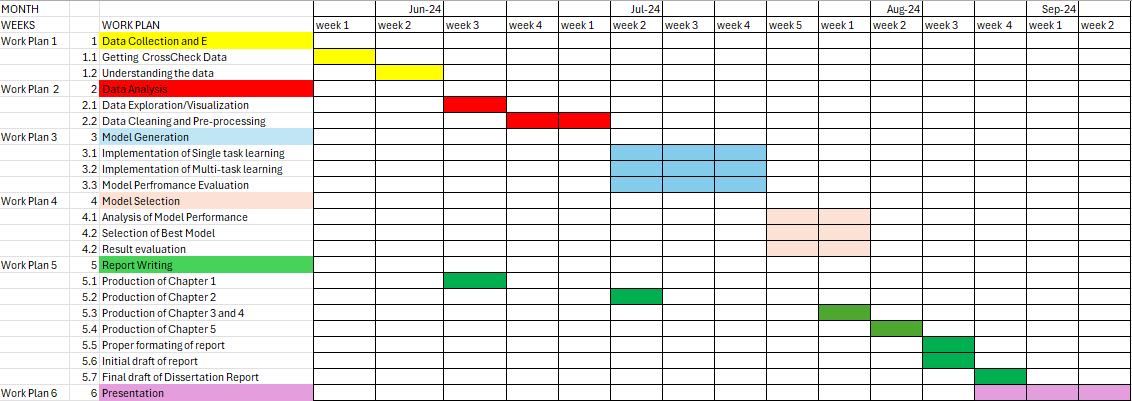
\includegraphics[scale=0.25]{work_plan.png}
\caption{Research Project Work Plan}
\label{work}
\end{figure}

\bigskip
\goodbreak


\section{Structure of Dissertation}
This dissertation is structured into five chapters, each progressively contributing to a comprehensive exploration of the research topic.

Chapter Breakdown
\begin{itemize}
\item Chapter 1: Introduction establishes the research context by outlining its background, motivation, and objectives.This outlines a clear framework for the dissertation.
\item Chapter 2:The Literature Review critically examines the existing body of research on machine learning applications across a range of mental health conditions, with a particular emphasis on its use in the prediction of Schizophrenia.Additionally, it explores the use of various both single-task and multi-task learning approaches, identifying knowledge gaps for further investigation.
\item Chapter 3: The Research Methodology section outlines the comprehensive approach taken to address the study’s objectives, which includes  data collection, pre-processing, and feature engineering. The section also covers both personalized and generalized modeling approaches, providing a thorough rationale for the chosen research design to ensure alignment with the study's goals.
\item Chapter 4: Results and Discussion presents the development and evaluation of generalized and personalized single-task and multitask learning models.Analyzes and discusses the performance comparison of these models.
\item Chapter 5: Conclusion summarizes key findings and assesses the achievement of research objectives. Discuss implications and provide recommendations for future research.
Each chapter is carefully structured to create a unified narrative that methodically tackles the research questions, providing a thorough and concentrated examination of the subject matter
\end{itemize}
\section{Summary}
The introduction chapter establishes the foundation for this research, which aims to compare the effectiveness of single-task learning (LassoCV) and multi-task learning (MultitaskLassoCV) models in predicting symptoms in Schizophrenia patients. Schizophrenia, a severe mental disorder, requires early and accurate detection to improve patient outcomes. This research is motivated by the need to develop more reliable diagnostic tools using multi-task learning which can lead to better and personalized treatment and overall patient well-being. Single-task learning, focusing on solving one specific task, and multi-task learning, which simultaneously addresses multiple related tasks, are the two approaches compared in this study. The hypothesis suggests that multi-task learning will provide superior diagnostic performance and generalization, especially given the complex nature of Schizophrenia. The dissertation is divided into five major chapters, each building on the previous chapters to give a comprehensive and in-depth exploration of the research topic. The subsequent chapters will cover a detailed literature review, methodology, results and discussion and conclusion.


%%% ----------------------------------------------------------------------

% ------------------------------------------------------------------------
% -*-TeX-*- -*-Hard-*- Smart Wrapping
% ------------------------------------------------------------------------
\def\baselinestretch{1}

\chapter{Literature Review}

\def\baselinestretch{1.44}

%%% ----------------------------------------------------------------------

This chapter reviews the related literature to my dissertation topic. 
   
\smallskip

%%% ----------------------------------------------------------------------
\goodbreak
\section{Review on basic methods}
Machine learning (ML) has significantly advanced various fields, including “computer vision, natural language processing(NLT), artificial intelligence, and speech recognition”. It allows developers and researchers to extract essential insights from datasets, deliver tailored experiences, and create advanced systems \citep{jordan2015machine}. Machine learning has facilitated rapid and extensive analysis of intricate data in areas such as bioinformatics \citep{luo2016big}. These approaches are now being implemented in mental health data, offering substantial potential to improve patient outcomes and enhance the comprehension of psychological disorders and their treatment \citep{shatte2019machine}.

\citet{jordan2015machine}Shivangi(2015) investigated the use of various ML algorithms to predict depression using routine survey data, examining the methodologies and outcomes to provide insights into the efficacy of these approaches. The study utilized routine survey data, which included questions about home and workplace environments, family history of mental illness, and personal health information. A variety of machine learning algorithms were used to determine the most effective method for predicting depression, which include: K-Nearest Neighbors (KNN), Boosting, Decision trees, Random forest, Logistic regression, and Bagging (Bootstrap Aggregating). The results demonstrated that ensemble methods, particularly Boosting with  accuracy of 81.75\%, and Random Forest with accuracy of 81.22\%, significantly outperformed other algorithms in predicting depression.

In addition, \citet{sau2017predicting} investigated the use of machine learning classifiers to predict depression in elderly citizens, aiming for early diagnosis and improved medical intervention using the WEKA data mining tool.  Data were collected from senior citizens in Kolkata.Geriatric Depression Scale and classifiers such as Logistic Regression, Bayes Net, Multilayer Perceptron (MLP), Decision Tree and  Sequential Minimal Optimization (SMO), were utilized for the prediction. The study found that Bayes Net provided the best overall performance in predicting depression, particularly when using the percentage split test option in WEKA. This approach promises to enhance early detection and treatment of depression among seniors, reducing the manual burden on healthcare providers. 

\citet{malik2023anxiety} explores the application of machine learning techniques to predict the severity levels of anxiety, depression, and stress among college students. The study used the DASS21 questionnaire to collect data from 400 students, classifying their responses into five severity levels: “normal, mild, moderate, severe, and extremely severe”. Machine learning algorithms, including Support Vector Machine (SVM), Decision tree, K-Nearest Neighbor (KNN), Naïve Bayes, and logistic regression were used to predict these mental health issues. Performance metrics such as F1 score, accuracy, recall, precision and specificity were used to evaluate the models, with a focus on addressing class imbalance. KNN emerged as the best-performing model with the highest accuracy and F1 score, making it the most effective in handling imbalanced data and predicting mental health severity accurately.

 \citet{haque2021detection} however studied the use of machine learning to detect depression in children and adolescents. Recognizing the profound impact of childhood depression on individuals, families, and society, the study sought to create an early detection model. The research utilized the Young Minds Matter (YMM) dataset involving 6,310 participants, which includes comprehensive data on Australian children aged 4-17. For the feature selection, the Boruta algorithm was combined with a Random Forest (RF) classifier. Eleven critical features were identified for detecting depression: unhappiness, sleep disturbance, suicidal thoughts, lack of fun, weight changes, irritable mood, fatigue, diminished interest, psychomotor changes, concentration issues, and the presence of any five of these symptoms. Tree-based Pipeline Optimization Tool (TPOT classifier) was used to select and optimize the tested models which included: Decision Tree (DT), Random Forest (RF), Gaussian Naive Bayes (GaussianNB), and XGBoost (XGB).  Among the models, Random Forest (RF) outperformed others, achieving 99\% precision and 95\% accuracy, with a runtime of 315 milliseconds. The study highlights the significance of parental and social involvement in a child's life and the adverse effects of family disruptions and poor health conditions on mental health.

Another notable mental health illness that machine learning helps to predict is Alzheimer. \citet{salunkhe2022prediction} in their study used Random Forests (RF) and Support Vector Machines (SVM) to develop predictive models for diagnosing Alzheimer's using the OASIS dataset. The OASIS dataset, containing MRI scans and other attributes, was used and it was observed that SVM achieved higher accuracy (93\%), precision, recall, and F1 score compared to RF. 


Suicide is also a major public health issue affecting millions globally, especially the youth. \citet{faisal2023machine} studied using machine learning (ML) to predict suicidal thoughts and behaviors. The dataset used in the research work was obtained from the “Global School-based Student Health Survey (GSHS)”  which includes data from teenagers across 26 countries. The data includes various attributes such as alcohol consumption, parental understanding, drug use, past suicide attempts and bullying experiences.  Machine learning models used in the research work include Support Vector Regression (SVR), Random Forest (RF), Linear Regression (LR), Ridge Regression (RR), K-Nearest Neighbors (KNN), Multi-Layer Perceptron (MLP), and Extreme Gradient Boosting (XGB). SVR was found to have the best performance with the lowest MAE (4.6588), MAPE (0.6561) and RMSE (4.6589), indicating it is the most suitable model for predicting suicidal behavior by analyzing various risk factors. The study highlights the potential of Machine Learning to significantly aid in suicide prevention efforts by providing early detection and intervention.

In his study, \citet{talaei2019predictive} investigated predicting multiple medical complications among patients with chronic diseases using predictive analytics. The data was mined from the Electronic medical records (EMRs) of 1078 patients with hypertrophic cardiomyopathy from 2009 to 2017. Models such as Support vector machines (SVM),  Decision trees (DT), Logistic regression (LR), and artificial neural networks (ANN) were used in predicting complications such as Heart failure, cardiac arrest and problems with heart valves. Independent Prediction of Multiple Complications (IPMC) involves the use of single-task learning (STL) to predict each complication independently whereas, Concurrent Prediction of Multiple Complications (CPMC) was used to predict complications concurrently, considering their interrelationships. The study compares these two methods and demonstrates that CPMC accounts for the interrelationships among complications.  Discrimination (AUC) and calibration (Q-Score) performance metrics were used and it was observed that CPMC outperforms in both discrimination, meaning its capability to differentiate between patients who will develop complications and those who will not, and calibration (the accuracy of the predicted probabilities). 
\citet{abdillah2021comparative} compared single-task learning (SLT) and Multi-task Learning(MLT) in the context of research protocol classification, particularly in the health domain, to aid the ethical review process by the ethical committee. The study utilized two datasets: one with 36 documents related to ethical protocols and another with 20,972 research paper summaries. The documents were processed and annotated for multiple labels indicating ethical issues and research topics. Although , the  MTL outperformed STL in terms of Hamming Loss (0.125 vs. 0.182 on the smaller dataset and 0.097 vs. 0.113 on the larger dataset) and Jaccard Score (0.785 vs. 0.720 on the smaller dataset and 0.635 vs. 0.571 on the larger dataset), but in terms of computation time, MTL was slower, taking 27\% more time on the smaller dataset and 41\% more time on the larger dataset. It was concluded that despite higher computational costs, MTL showed better performance in multi-label classification tasks. 

\section{Related Work}
\subsection{Single-task Learning}  
The Cross Check study represents a significant step toward the development of passive sensing systems for mental health monitoring. It underscores the potential of leveraging smartphone technology to enhance the care and management of individuals with schizophrenia through early detection and intervention strategies. \citet{wang2016crosscheck}  initiated the first attempt to address the pressing need for early prediction of mental health changes in individuals diagnosed with severe mental illness, with a particular emphasis on those suffering from schizophrenia. 21 outpatients with schizophrenia were monitored after hospital discharge over a period of 2-8.5 months. Smartphones collected passive sensor data, including information on sleep, phone usage, conversations and mobility and participants completed periodic self-reports on their mental health. The study analyzed the correlation between passive sensor data and self-reported Ecological Momentary Assessment(EMA). Inference models were built to predict mental health scores with a mean error of 7.6\%.  Statistically significant associations were found between passive behavioral features and self-reported EMA.The study demonstrated that models could predict mental health scores accurately by leveraging data from the population and adapting to individual-specific data. Personalized models required fewer data points to adapt quickly to new users.  The predictive models were able to achieve a mean absolute error (MAE) of 1.378 for positive scores and 1.383 for negative scores, with strong correlations (r values) between predicted and actual scores. 

In 2017,\citet{wang2017predicting} advanced the research by utilizing mobile phone sensor data to predict the severity of symptoms as assessed by the Brief Psychiatric Rating Scale (BPRS). The system predicts weekly scores on a 7-item Brief Psychiatric Rating Scale (BPRS), assessing symptoms like grandiosity, hallucinations and more. The study compares the predictive accuracy of models using passive sensing, EMA and a combination of both. The best results achieved a mean absolute error (MAE) of 1.45, showing a strong correlation between predicted and actual BPRS scores. The system identifies at-risk patients based on score thresholds and trends, enabling timely clinical interventions. The research highlights the potential of mobile sensing for continuous symptom monitoring, although it notes limitations such as an unbalanced dataset and the need for more data from patients with severe symptoms. Future improvements include better training models with additional high-severity data and addressing generalization to different environments. However, \citet{wang2020predicting} study addresses challenges in predicting rare events in a longitudinal dataset and finds the best prediction results using principal components (PCA) from both passive sensing and self-reports with 30-day prediction windows. 

In their research, \cite{adler2020predicting} utilized two distinct encoder-decoder neural network architectures in combination with a clustering-based local outlier factor model to forecast behavioral deviations during the 30-day period leading up to a relapse, referred to as the near relapse period. The models were trained to replicate behaviors representative of "days of relative health" (DRH), which occur outside this near relapse window. Following this, a post hoc analysis was conducted using the most effective model to identify behavioral traits that significantly contributed to distinguishing anomalies near relapse from DRH. This analysis focused on four participants who experienced multiple relapses during the study. The most successful model, a fully connected neural network autoencoder, demonstrated a median sensitivity of 0.25 (interquartile range: 0.15-1.00) and a specificity of 0.88 (interquartile range: 0.14-0.96), indicating a 108\% improvement in the median detection of behavioral anomalies near relapse. The proposed approach was more effective in predicting anomalies among patients with Serious Mental Health Disorders (SSDs) in the 30 days preceding relapse and can be applied to identify behavioral changes leading up to relapse events. 

However, \citet{lamichhane2022psychotic}introduces RelapsePredNet, a personalized Long Short-Term Memory (LSTM) neural network-based model for predicting psychotic relapse in schizophrenia patients using mobile sensing data. Leveraging continuous mobile sensing data from 63 schizophrenia patients in the CrossCheck dataset, the model demonstrated substantial enhancements in prediction accuracy compared to current approaches. The personalized RelapsePredNet model outperformed non-personalized versions and existing anomaly detection models. Personalization was crucial for improving prediction accuracy, and the study opens avenues for further research into personalized and real-time monitoring systems for mental health management.
\subsection{Multi- task Learning}
Previous research by \citet{adler2020predicting} focused on data from single studies with homogeneous populations and short periods, limiting model applicability to broader contexts. In a recent study, \citet{adler2022machine} merged data from the CrossCheck study, involving schizophrenia patients, and the StudentLife study, focused on university students, to evaluate whether models trained on this combined dataset offer better prediction accuracy than those trained on data from just one of the studies. Models trained with combined data from both studies showed better prediction performance than those trained on single-study data. Gradient Boosting Regression Trees (GBRT) were utilized to forecast mental health symptoms, while hyperparameters such as the learning rate, the number of trees, and the depth of the trees were modified. In addition, personalization and oversampling techniques were applied to enhance model accuracy. The research shows that machine learning models, when trained on integrated data from various diverse studies, are capable of effectively generalizing across different populations and settings.

Moreover, \citet{tseng2020using} explores the prediction of schizophrenia symptom progression through the application of "behavioral rhythms and multi-task learning (MTL) models." The research employed MTL to forecast ecological momentary assessment scores across ten distinct symptoms. Results indicated that MTL models outperformed single-task learning models in accurately predicting the trajectories of individual symptoms, including emotional states such as depression, auditory hallucinations, sociability, and calmness. In addition, the models enhanced interpretability by accounting for participant similarities and differences in symptom manifestation. Unsupervised clustering further identified unique subtypes within each symptom category based on feature weights. These findings have substantial clinical implications, supporting early detection and intervention strategies without imposing additional burdens on patients or clinicians.

In conclusion, the literature reviewed consistently supports the notion that multi-task learning (MTL) outperforms single-task learning (STL) in various applications, particularly in the context of predicting complex symptom trajectories. This alignment across studies underscores the robustness and generalizability of MTL models in handling interconnected tasks, such as the prediction of multiple schizophrenia symptoms. The collective evidence highlights that MTL not only enhances predictive accuracy but also improves the interpretability of the models by accounting for the relationships between different tasks. This consensus among the literature directly aligns with the research objectives of this work, which aims to investigate the superior performance of MTL over STL for predicting EMA score. The findings of this study will contribute to this body of knowledge by using a model that has both variants of SLT and MLT to verify whether MTL models will provide a more effective approach for forecasting individual Schizophrenia symptom progressions, ultimately supporting the advancement of more nuanced and targeted clinical interventions.

\section{Summary} 
The review of literature in this chapter has revealed the consensus between different study that multi-task learning outperforms single-task learning for the prediction of various health-related conditions such as Depression, Alzheimer, Suicide and also Schizophrenia. In multi-task learning, the model is trained simultaneously by sharing of information across multiple related tasks, whereas in single-task learning, each task is trained independently and without interaction, thus not benefiting from shared information. The findings demonstrate that the sharing of information between multiple related tasks in multi-task learning significantly enhances the overall generalization performance of the model. Additionally, multi-task learning has proven to be more resource-efficient, as it enables the simultaneous training of multiple tasks, thereby eliminating the necessity for individual models for each task. However, it is important to acknowledge that despite its efficiency in resource utilization, multi-task learning can be more computationally expensive due to the complexity involved in managing and optimizing several tasks concurrently. This added complexity may require more sophisticated infrastructure and extended training times, which could be considered a trade-off for the enhanced performance and interpretability that MTL provides. This advantage is particularly pronounced in the context of mental health conditions such as schizophrenia. Multi-task learning enables the integration of various related tasks, including symptom prediction, treatment response, and patient outcome monitoring, into a unified and comprehensive model. By capitalizing on the interconnected nature of these tasks, multi-task learning can significantly enhance predictive accuracy and treatment effectiveness, offering a more holistic approach to managing and understanding schizophrenia. Overall, this chapter highlights the superior performance of multi-task learning compared to single-task learning, emphasizing its broader applicability in diverse machine learning scenarios, with a special focus on its effectiveness in mental health applications like schizophrenia.

   


\def\baselinestretch{1.66}
\medskip


%%% ----------------------------------------------------------------------

% ------------------------------------------------------------------------
% -*-TeX-*- -*-Hard-*- Smart Wrapping
% ------------------------------------------------------------------------
\def\baselinestretch{1}

\chapter{Methodology Design}

\def\baselinestretch{1.44}

%%% ----------------------------------------------------------------------

This chapter outlines the methodology developed for my dissertation project. 
   
\smallskip

%%% ----------------------------------------------------------------------
\goodbreak
\section{Analysis of the methods}
The core hypothesis of this study is that MultiTaskLassoCV, will outperform single-task learning (LassoCV) in both accuracy and robustness. By applying an L1-norm regularization, LassoCV penalizes the absolute size of coefficients, encouraging sparsity in the model, which can enhance interpretability. However, while LassoCV is effective for single-task learning, it might not fully exploit the inherent relationships between different mental health indicators in schizophrenia \citep{tibshirani1996regression}. MultiTaskLassoCV extends LassoCV to a multi-task framework, allowing simultaneous training across multiple related tasks. This approach is particularly advantageous in the context of mental health prediction, where symptoms are often interrelated. By leveraging these relationships, MultiTaskLassoCV is anticipated to yield superior performance in predicting schizophrenia-related mental health conditions, both in terms of accuracy and robustness (\citep{zhou2011malsar} and \citep{tseng2020using}). 

For a given user's data~\(X_{u} \in \mathbb{R}^{e_{u} \times d}\) and the EMA symptom scores \(Y_u^s \in \mathbb{R}^{e_{u}}\)  the objective is shown below: 

\[\min_{W_u^s} \| Y_u^s - X_u W_u^s \| + \alpha | W_u^s|_{1}\] u represents the user, \(e_{u}\)  represents the number of EMA entries by the user, d is the feature vector dimension, s is the symptom and  \(\alpha\) controls the sparsity of \(w_u^s\), higher \(\alpha\) values result in fewer non-zero coefficients.

The weight vector is represented by : \(w_u^s \in \mathbb{R}^d\) and it's used for predicting symptom s for user u, while the \(l_{1}\)-norm\(|W_u^s|_{1}\) = \sum{i}\ |w_{ui}^s|

The magnitude of these coefficients indicates the importance of each feature in predicting EMA scores. However, for the generalized model where a single model is used to predict all the users, the objective function is shown below : 

\[\min_{W^s} \| Y^s - X W^s \| + \alpha | W^s|_{1}\] where
\(X =[X_{1} & \cdots & X_{p} ]\in \mathbb{R} ^{(\sum_{u=1}^{p} e_u\ )}\) denotes the combined feature matrix for users 1,2,3 to
p and \(Y^s =[Y^s_{1} & \cdots & Y^s_{p} ]\in \mathbb{R} ^{(\sum_{u=1}^{p} e_u\ )\times d}\) denotes combined EMA scores for symptom s across all patients and \(w_u^s \in \mathbb{R}^d\), which is the weight vector.

For multi-task learning, a given user's EMA scores across various symptoms is represented as \(Y_u = [Y^1_{u} & \cdots & Y^k_{u} ] \in \mathbb{R}^{eu \times k}\) 
where k denotes the total number of symptoms. The objective function for MTL is defined based on the approaches outlined by \citet{nie2010efficient} and  \citet{zhou2011malsar} as shown below :
\[\min_{W_u} \| Y_u - X_u W_u \|_F^2 + \alpha \| W_u \|_{2,1}\]


\(W_u = [W^1_{u} & \cdots & W^k_{u} ]\in \mathbb{R}^{d \times k} \) serves as the weight matrix used for predicting individual symptom scores. The regularization parameter is denoted by \(\alpha\), and \(||.||_F\) represents the Frobenius norm. \(.|| W ||_{2,1}\)  term is calculated as \(\sum\_{i}  \sqrt{\sum_{j} w^2_{i\j} }\) reflecting  \(l_{2,1}\)-norm, which is effective in promoting joint group sparsity by encouraging related tasks to share a limited set of features \citep{tseng2020using}.

 Generalized modeling for both auto selection and hyperparameter tuning for Single-Task Learning (STL) and Multi-Task Learning (MTL) were examined. For personalized modeling, sufficient data is crucial, which is a limitation of this dataset. To confirm the assumption regarding data sufficiency, personalized modeling was performed, and the results from participants with the highest and lowest number of entries—study\_id 47 and study\_id 70, respectively—were evaluated. This selection was used to compare the performance of STL and MTL approaches across all symptoms. Due to computational constraints, only the automatic feature selection using LassoCV and MultitaskLassoCV were evaluated.
 
 The decision to use MultitaskLassoCV and LassoCV over alternatives like Ridge regression, ElasticNet, or other multi-task learning methods, is based on its ability to promote joint sparsity and improve prediction accuracy in high-dimensional settings, which is critical for the nuanced detection of schizophrenia-related conditions.


\section{Design of Methodology}
This section outlines the steps taken to prepare, ensuring robust and reliable model development.
\subsection {Data Exploratory Analysis and Visualization} 
\subsubsection{Data Source} 
The data used for this study was provided by my supervisor Dr.Min Aung, who was part of the team that carried out the CrossCheck research \citep{wang2016crosscheck}, ensuring compliance with ethical standards and data privacy regulations. The dataset spans January 21, 2015, to April 20, 2017.

\subsubsection{Data Features} 
The dataset comprises 155 features across 23,573 rows, including behavioral metrics divided into four six-hour intervals each day to capture daily patterns. The features include 57 numeric (float) features, 97 numeric (integer) features and 1 categorical feature. The data includes key behavioral metrics such as conversation frequency, movement activities (e.g., vehicle, bike, foot), and self-reported Ecological Momentary Assessment (EMA) scores, which are critical for understanding the mental health states of the participants as shown in Figure \ref{feat} and Table 3.1

\begin{figure}[H]
    \centering
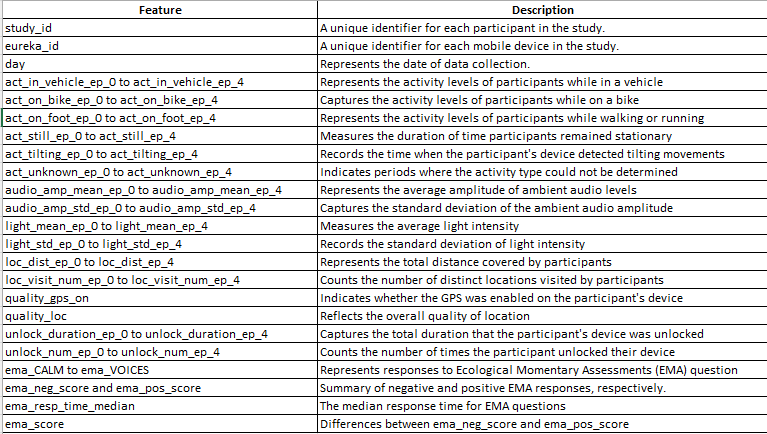
\includegraphics[scale=0.50]{feature.png}
\caption{Data Features}
\label{feat}
\end{figure}

\bigskip
\goodbreak
    
\smallskip
\begin{table}[H]
\centering
\caption{ 10 EMA questions as extracted from \citet{wang2016crosscheck}}
\begin{tabular}{|l|}
\hline
\textbf{Questions} \\ \hline
Have you been feeling CALM? \\ \hline
Have you been SOCIAL? \\ \hline
Have you been bothered by VOICES? \\ \hline
Have you been SEEING THINGS other people can’t see? \\ \hline
Have you been feeling STRESSED? \\ \hline
Have you been worried about people trying to HARM you? \\ \hline
Have you been SLEEPING well? \\ \hline
Have you been able to THINK clearly? \\ \hline
Have you been DEPRESSED? \\ \hline
Have you been HOPEFUL about the future? \\ \hline
\textbf{Options:} 0- Not at all; 1- A little; 2- Moderately; 3- Extremely. \\ \hline
\end{tabular}
\end{table}

\smallskip
 \subsubsection{Descriptive Statistics } 
Descriptive statistics was implemented to assess the variability in participants' activities and the EMA. Correlation analysis was conducted to explore the relationships between different (EMA) scores and other variables. Outliers were detected using the z-score method, and a thorough analysis of missing values was performed to identify features with incomplete data. Additionally, the consistency of aggregated scores was verified by ensuring that the sum of scores for epochs 1 through 4 matched the total score for epoch 0.


\subsection{Data Cleaning} 
The `Eureka\_id` column was excluded as it has no impact on the analysis. In addition, all aggregated features (e.g., `epoch\_0`) were excluded from the dataset due to mismatched aggregated scores to enhance the data quality.  The refined dataset now comprises 126 features and 12,232 observations, ensuring a robust foundation for analysis.
 \subsubsection{Handling Missing Values}
To handle missing values in targets which are the 10 symptoms, backfilling was applied with a limit of three days as the EMA questions and responses were gotten within 2 to 3 days. Interpolation and removal of remaining missing values were also examined, in addition to mean imputation and removal of rows with missing values for other variables. Among all the methods evaluated, backfilling missing EMA values within a three-day window and subsequently removal of outstanding missing data method was adopted for the data cleaning as it performed better. This observation aligns with the assumptions made by \citet{adler2020predicting}, who suggest that interpolation methods can introduce bias by smoothing data towards mean values. This bias may obscure subtle variations in the data, thereby limiting the ability of models to accurately identify changes indicative of mental health status.
\subsubsection{Handling Outliers}
Outliers, particularly in the "day" column, were addressed by removing data that fell outside the study period (e.g., entries from 1969), which likely resulted from device configuration errors.
\subsection{Feature engineering}
In the crosscheck dataset, different columns such as audio\_conversations, location\_distance, sms\_in,call\_duration have varying scales.Using these features without normalizing them to a uniform scale could introduce bias into the model. The StandardScaler was applied for feature standardization, ensuring all features contribute equally to the model, preventing any single feature from disproportionately influencing the results due to its scale. This is particularly useful for linear regression algorithms like LassoCV that are sensitive to the scale of the input features \citep{mayer1974procedures} and \citep{mathur2023generalized}

 \subsubsection{Cross-Validation}
Cross-validation is a pivotal component in refining the LassoCV model, particularly for schizophrenia prediction. This method involves partitioning the dataset into \( k \) subsets, known as folds, allowing the model to be trained and validated systematically. The process is repeated \( k \) times, with each fold serving once as the validation set and the remaining \( k-1 \) folds as the training set. This iterative approach not only aids in identifying the optimal regularization parameter, \(\alpha\), but also ensures a model that strikes a balance between accurately fitting the training data and generalizing to new, unseen data \citep{kolluri2020reducing}

In the context of schizophrenia research, where overfitting can result in misleading conclusions, cross-validation enhances model reliability and predictive power, especially when forecasting Ecological Momentary Assessment (EMA) outcomes. Furthermore, integrating an 80-20\% data split with cross-validation adds an extra layer of validation: after the model is optimized on 80\% of the data using cross-validation, the remaining 20\% serves as a hold-out set, providing an independent test of the model’s performance on entirely new data. This study also explored hyperparameter tuning for the \(\alpha\) value, comparing manually tuned results with those automatically selected by LassoCV. This comparison underscores LassoCV's robust framework for developing predictive models, highlighting its potential to optimize predictive accuracy and clinical utility. 

\section{Evaluation Methods and Measures}
In mental health, large prediction errors can have serious implications. For example, underestimating the severity of a patient's condition might lead to inadequate care, while overestimating it might result in unnecessary interventions. RMSE's sensitivity to large errors ensures that models are penalized more for these significant mistakes, promoting the development of models that minimize these critical errors. The RMSE value is in the same unit as the outcome being predicted. This is particularly important in mental health, where clinicians and stakeholders often need to understand model performance in practical, understandable terms. In addition, mental health data often involves significant variability due to individual differences in symptom presentation and response to treatment. RMSE’s penalization of variance in errors helps ensure that the model does not produce predictions with wide variability, which could lead to inconsistent or unreliable assessments. This is crucial in mental health, where consistency in evaluation is vital for accurate diagnosis and treatment planning. Also,mental health datasets can include outliers, such as extreme cases of severe mental health conditions. RMSE's sensitivity to these outliers ensures that the model does not ignore or overly smooth out these critical cases. In mental health, where extreme cases often need more attention, having an evaluation metric that highlights poor performance in these areas is beneficial. Using RMSE as an evaluation metric for mental health datasets is justified due to its ability to highlight significant errors, maintain interpretability, and manage variability in predictions. In the context of Schizophrenia,  where accurate prediction and consistency are paramount, RMSE helps ensure that models perform reliably across a range of cases, including those with extreme outcomes. This makes RMSE a valuable tool for evaluating and improving predictive models in mental health research and practice \citet{zhang2024students}.

To test for the significance of the difference between the STL and MTL were examined using the Wilcoxon test. The Wilcoxon test was selected for comparison because it is a non-parametric test, meaning it does not require the assumption of normality in the dataset. Additionally, it is ideal for comparing the performance of STL and MTL models on the same set of targets, and it is well-suited for small sample sizes \citep{tseng2020using}


\section{Tools and Resources}
The research was conducted using a variety of tools and resources that supported efficient data processing and accurate analysis. They include :
\begin{itemize}
    \item Programming Languages: Python was the primary language used due to its robust data science libraries and widespread adoption in machine learning.
    \item Libraries and Frameworks: Pandas and NumPy were used for data manipulation and processing. Scikit-learn was employed for implementing machine learning algorithms and conducting model evaluations. Matplotlib and Seaborn facilitated detailed data visualizations, important for understanding data distributions and model outcomes.
   \item Development Environments: Although Jupyter Notebook and Google Colab were used as they provide an interactive environment for coding and visualization, Google Colab was chosen for its cloud-based computing capabilities, enabling efficient handling of computationally intensive tasks and providing access to GPU acceleration when needed.
   \item Data Resources: The dataset was provided by my supervisor, ensuring its relevance and quality, tailored specifically to the research objectives.
\end{itemize}

These tools and resources were instrumental in ensuring the smooth execution of the project, from data preprocessing to model evaluation

\section{Summary} 
This chapter outlined the methodology used to evaluate the hypothesis of this study that      MultiTaskLassoCV would outperform LassoCV in detecting schizophrenia-related mental health symptoms. The analysis of methods highlighted the advantages of MultiTaskLassoCV in handling complex, multifaceted data. The design of the methodology detailed the steps taken to prepare the data, including exploratory analysis, data preprocessing, and feature engineering. RMSE evaluation metrics was chosen to balance precision and interpretability, while the tools and resources section underscored the critical role of Python, Scikit-learn, and various visualization libraries.

   

\def\baselinestretch{1.66}
\medskip

%%% ----------------------------------------------------------------------

% ------------------------------------------------------------------------
% -*-TeX-*- -*-Hard-*- Smart Wrapping
% ------------------------------------------------------------------------
\def\baselinestretch{1}

\chapter{Result, Evaluation and Discussion}
\section{Exploratory Analysis Result}
\subsection{Exploratory Analysis }
\subsubsection{Data Distribution}
\begin{figure}[H]
    \centering
    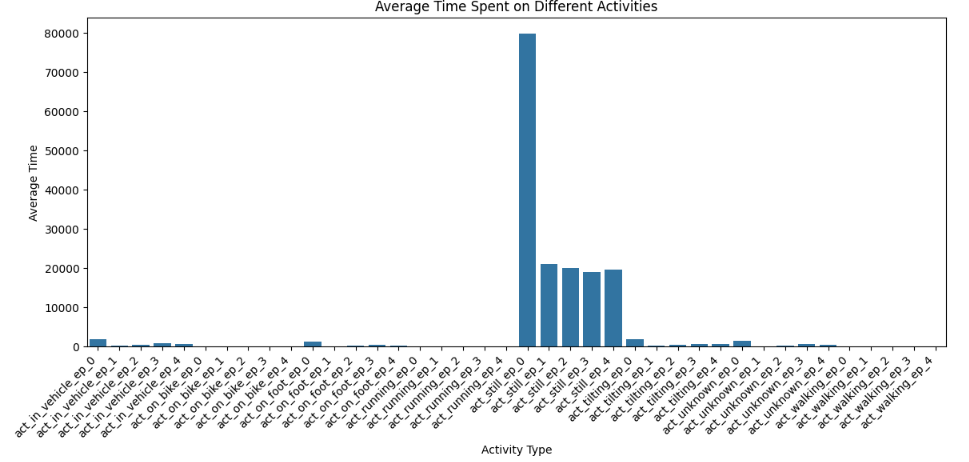
\includegraphics[width=0.5\linewidth]{Dissertation 24/activity.png}
    \caption{Activity Distribution}
    \label{fig:activ}
\end{figure}

\begin{figure}[H]
    \centering
    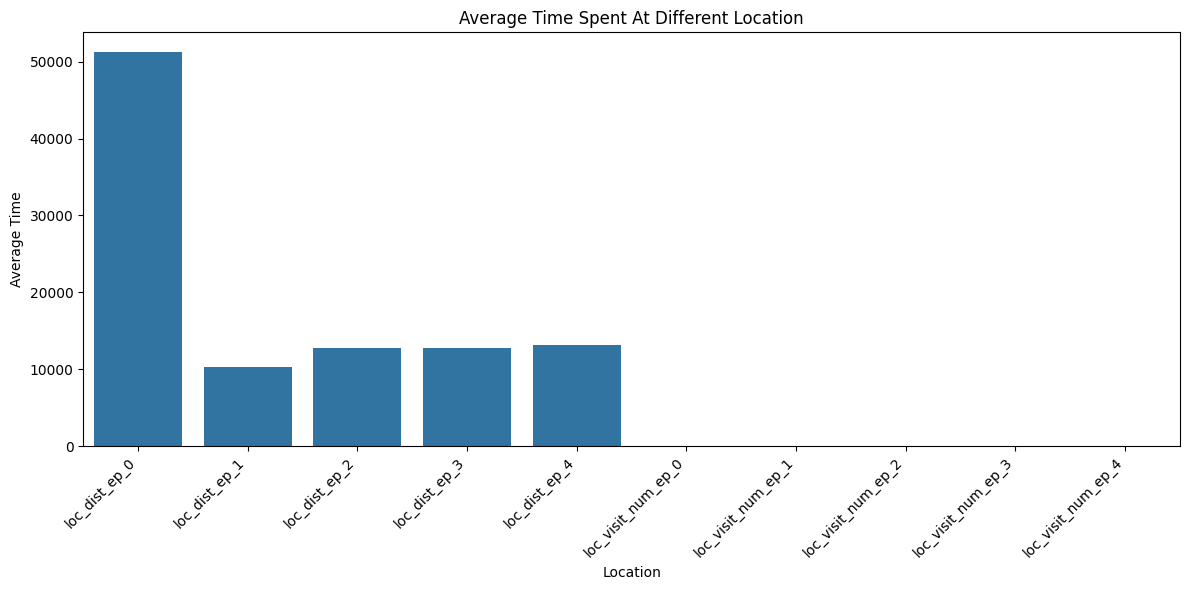
\includegraphics[width=0.5\linewidth]{Dissertation 24/loca.png}
    \caption{Location Distribution}
    \label{fig:loca}
\end{figure}

\begin{figure}[H]
    \centering
    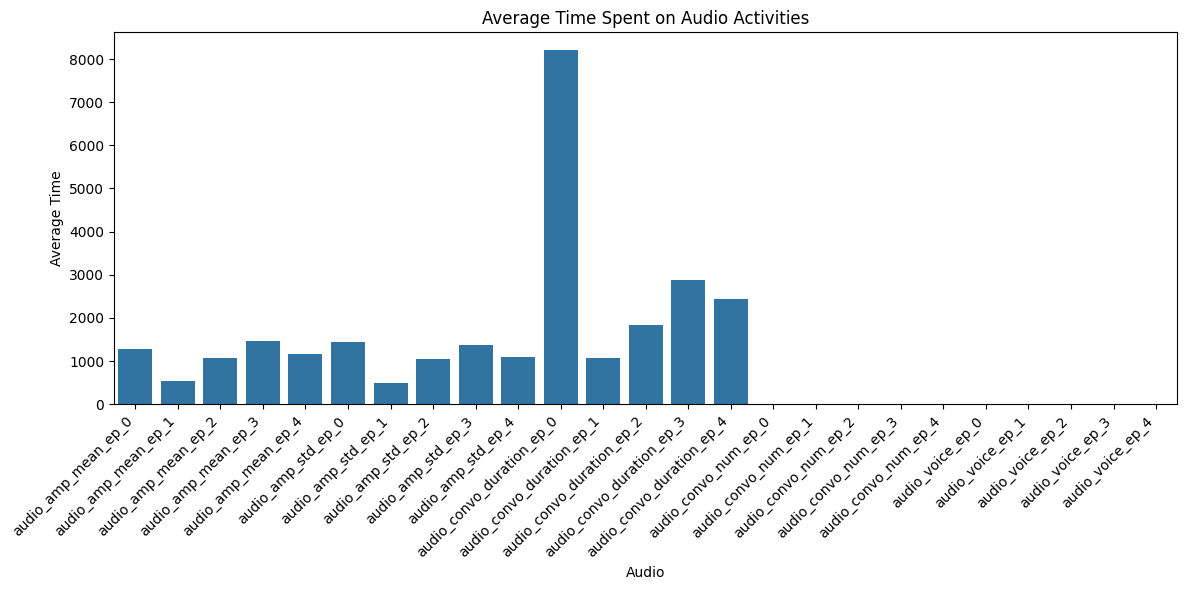
\includegraphics[width=0.5\linewidth]{Dissertation 24/activt.png}
    \caption{Audio Distribution}
    \label{fig:audio}
\end{figure}
From Figures \ref{fig:activ}, \ref{fig:loca} and \ref{fig:audio},  it can be observed that most activities peak during the 12-18 hour period (12 PM to 6 PM) which aligns with typical patterns of increased movement and activity during the day, while The 'still' activity peaks during the 0-6 hour period (12 AM to 6 AM), which aligns with typical sleeping hours. This analysis provides a more accurate representation of activity patterns throughout the day, correctly divided into four 6-hour blocks. It shows clear variations in activity levels across different times of the day, with most physical activities peaking in the afternoon, and stationary activity peaking during the night

\subsubsection{Descriptive Statistics}
\begin{figure}[H]
    \centering
    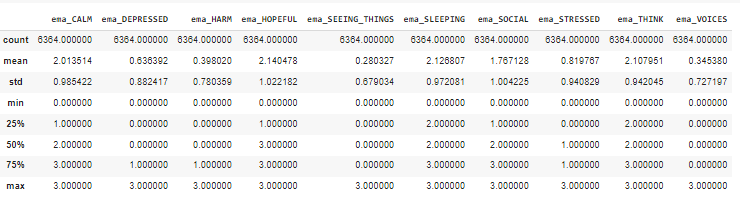
\includegraphics[width=0.5\linewidth]{descript.png}
    \caption{Descriptive Statistics For EMA}
    \label{fig:descr}
\end{figure}

From \ref{fig:descr}, it can be observed that participants generally reported feeling calm (mean = 2.02) and hopeful (mean = 2.14), with moderate variability in these experiences. Depression, self-harm thoughts, and hallucinations were relatively uncommon, though some participants did report higher levels of these issues, as indicated by the higher standard deviations. Overall, the positive EMA score was higher than the negative EMA score, suggesting participants experienced more positive than negative experiences, though there was notable variability in both. 

\subsubsection{Correlation Analysis}
\begin{figure}[H]
    \centering
    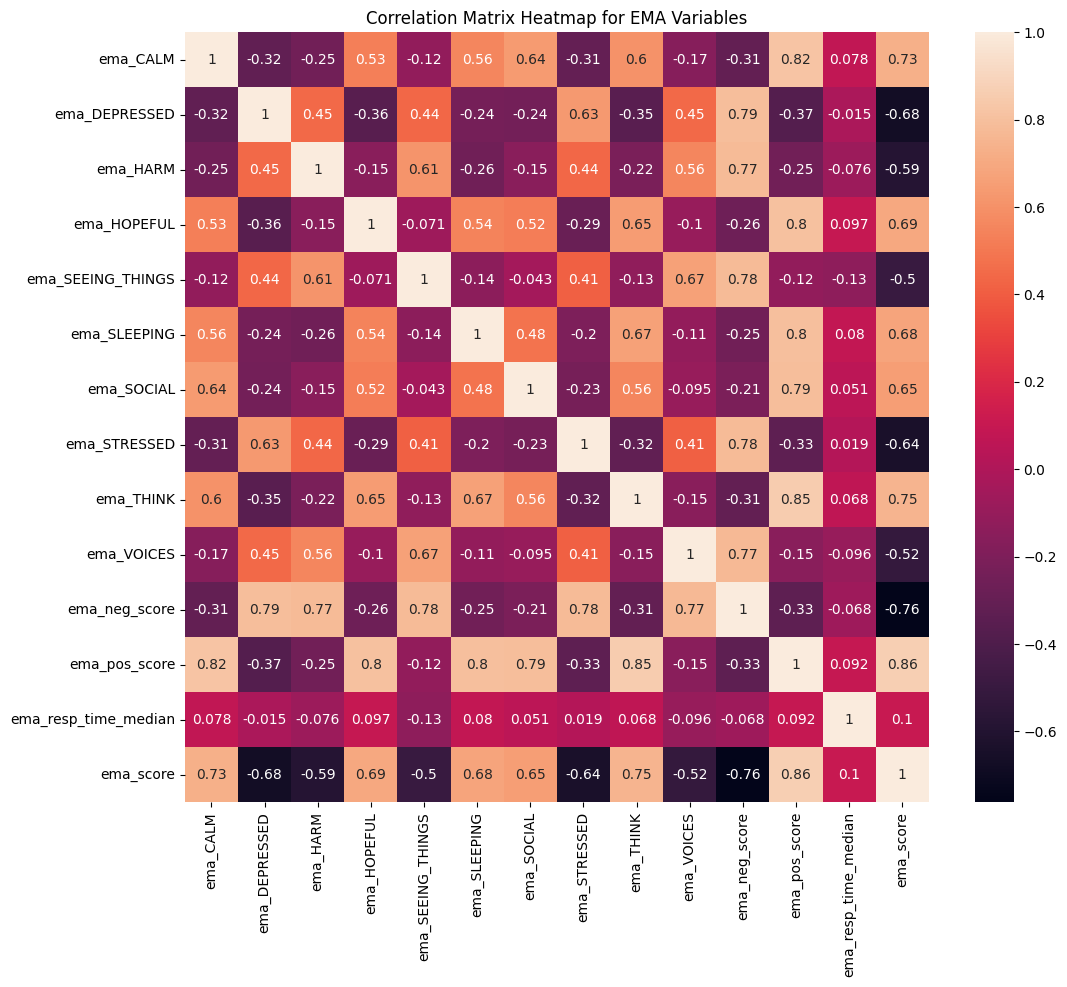
\includegraphics[width=0.5\linewidth]{Dissertation 24/heatmap.png}
    \caption{Correlation Analysis of EMA}
    \label{cor}
\end{figure}
\begin{figure}[H]
    \centering
    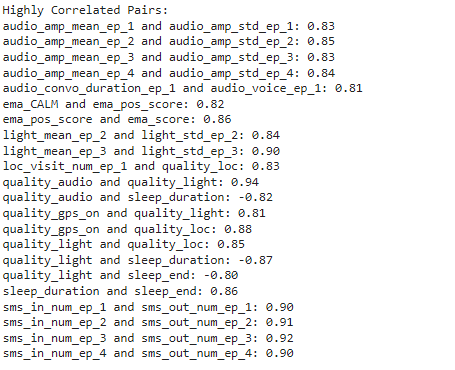
\includegraphics[width=0.5\linewidth]{Dissertation 24/high_correlation.png}
    \caption{Correlation of other features}
    \label{corr}
\end{figure}

Figure \ref{cor} and \ref{corr} illustrate the correlation between the EMA and also highlight significant correlations among other features. The EMA (positive, negative, and score) demonstrates a strong positive and negative correlation across all target variables. Specifically, EMA\_positive correlates highly with positive symptoms, while EMA\_negative correlates strongly with negative symptoms. These columns were dropped as they are aggregated results of the various positive and negative scores.
Due to the high degree of multicollinearity generally within the dataset as shown in \ref{corr}, feature selection is essential and this observation further justifies the application of the LassoCV models, which is well-suited for addressing multicollinearity and improving model performance.
\subsubsection{Outlier Detection}




\begin{figure}[H]
    \centering
    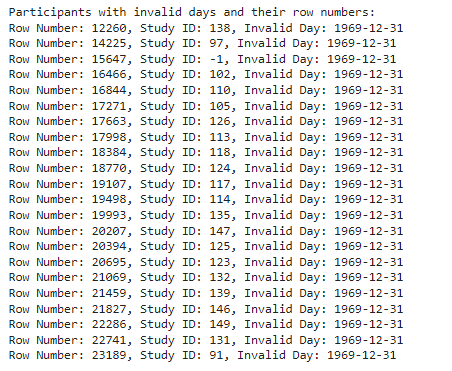
\includegraphics[width=0.5\linewidth]{Dissertation 24/correlation.png}
    \caption{Identified Outlier}
    \label{outler2}
\end{figure}
Using the z-score, a total of 10,002 outliers were detected. The z-score method was chosen because it standardizes the data, making it easier to identify significant deviations, which is crucial in health-related datasets. While these outliers will not be removed as they may represent important clinical variations, an exception is made for an outlier in the "day" column, where the year is recorded as 1969 as shown in Figure \ref{outler2}. This outlier was removed, as the dataset only covers the years 2015 to 2017.

\subsubsection{Missing values and Mismatched Aggregate Score}

\begin{figure}[H]
    \centering
    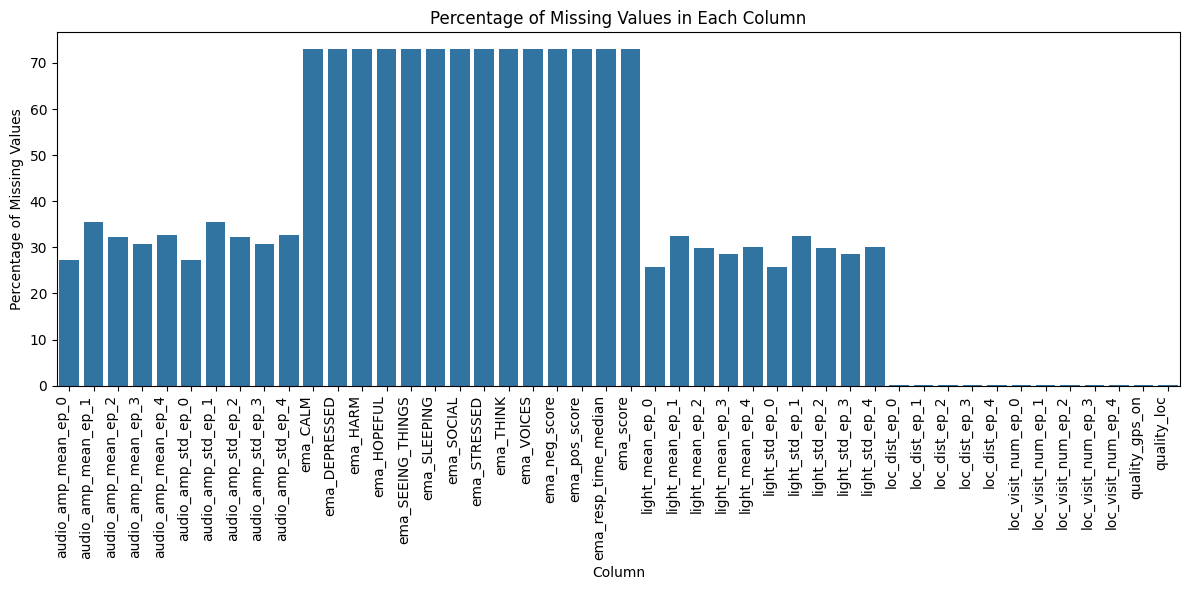
\includegraphics[width=0.5\linewidth]{Dissertation 24/missing values.png}
    \caption{Missing Value Percentage}
    \label{miss}
\end{figure}


\begin{figure}[H]
    \centering
    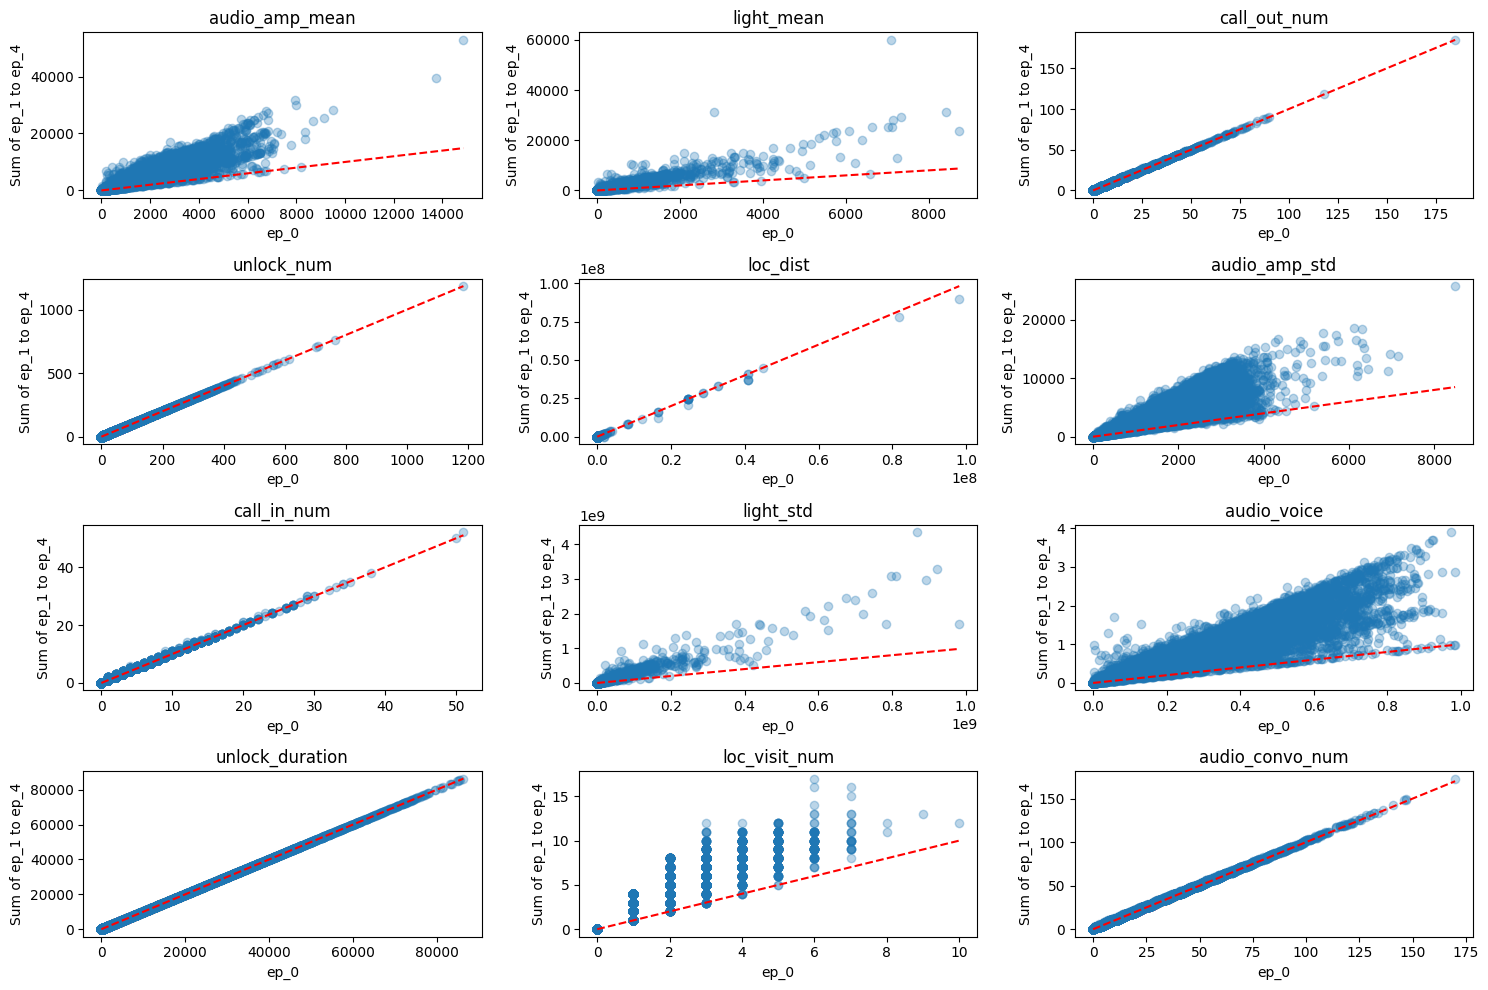
\includegraphics[width=0.5\linewidth]{Dissertation 24/ep_0.png}
    \caption{Aggregated Score for Epoch_0}
    \label{aggr}
\end{figure}

 Figure \ref{miss} illustrates the percentage of the missing data in the datasets while the scatter plots as shown in figure \ref{aggr} visualize the differences among the values in epoch 0 (ep\_0) and the sum of epoch 1-4 for each selected column.The discrepancies between the aggregated episode values and the reported totals (ep\_0) raise concerns about the reliability of the data. Since the summed values do not consistently align with ep\_0, it suggests potential data integrity issues that could negatively impact the analysis or modeling process, the columns were dropped to help avoid potential biases that could skew the results.

\section{Experimental Results}


\subsection{Evaluation of Results For Generalized Model }

\subsubsection{Evaluation of 5 Positive }


\begin{table}[H]
\centering
\caption{RMSE\_STL\_POST\_ and RMSE\_MTL\_POST\_ WITH TUNING}
\label{table:rmse_post_comp_tune}
\begin{tabular}{|l|c|c|}
\hline
\textbf{SYMPTOM} & \textbf{RMSE\_STL\_POST\_} & \textbf{RMSE\_MTL\_POST\_} \\ \hline
CALM & 0.9440423186838058 & 0.9437969762205503 \\ \hline
HOPEFUL & 0.9801633765713665 & 0.9787655753442269 \\ \hline
SLEEPING & 0.9335335511267163 & 0.9326096037267695 \\ \hline
SOCIAL & 0.9542377679345595 & 0.951665717565537 \\ \hline
THINK & 0.9077647518533615 & 0.9073883664439428 \\ \hline
\end{tabular}
\end{table}


\begin{table}[H]
\centering
\caption{RMSE\_STL\_POST and RMSE\_MTL\_POST AUTOMATIC }
\label{table:rmse_post_compP_auto}
\begin{tabular}{|l|c|c|}
\hline
\textbf{SYMPTOM} & \textbf{RMSE\_STL\_POST} & \textbf{RMSE\_MTL\_POST} \\ \hline
CALM & 0.9440290814743473 & 0.9440282511137151 \\ \hline
HOPEFUL & 0.9801637416300867 & 0.9788070117579115 \\ \hline
SLEEPING & 0.9337375219713796 & 0.9327292322207583 \\ \hline
SOCIAL & 0.953966732943221 & 0.9518563150050731 \\ \hline
THINK & 0.9076004187270317 & 0.9074626012701574 \\ \hline
\end{tabular}
\end{table}



Table \ref{table:rmse_post_comp_tune} and \ref{table:rmse_post_compP_auto} displays the result of the RMSE values for positive symptoms (ema\_CALM, ema\_HOPEFUL, ema\_SLEEPING, ema\_SOCIAL, and ema\_THINK) using automatic selection and hyperparameter tuning approach. The RMSE values across symptoms suggest comparable performance between the MTL and STL models, indicating that the models’ inbuilt structures are fairly robust even without parameter fine-tuning. However, notable observations include slightly higher RMSE values for symptoms like ema\_HOPEFUL and ema\_SOCIAL, suggesting these symptoms are inherently more challenging to predict accurately without hyperparameter tuning.
For hyperparameter tuning, the RMSE values for MTL and STL show slight improvements across all symptoms, indicating that hyperparameter tuning effectively reduces the prediction error and enhances model accuracy.
A notable improvement can be seen particularly in the symptoms where automatic selection had higher RMSE values (ema\_HOPEFUL and ema\_SOCIAL), suggesting that tuning helps the models better capture the complexities associated with these symptoms.

Overall, it can be observed that MTL in ema\_SOCIAL significantly outperforms STL, demonstrating a clear benefit in predicting social engagement, likely due to MTL’s ability to generalize better by learning from related tasks.

\subsubsection{Evaluation of 5 Negative}

\begin{table}[H]
\centering
\caption{ RMSE\_STL\_NEGT and RMSE\_MTL\_NEGT AUTOMATIC SELECTION}
\label{table:rmse_negt_comparison}
\begin{tabular}{|l|c|c|}
\hline
\textbf{SYMPTOM} & \textbf{RMSE\_STL\_NEGT} & \textbf{RMSE\_MTL\_NEGT} \\ \hline
DEPRESSED & 0.8707861943261692 & 0.8709503395531324 \\ \hline
HARM & 0.7338423144323089 & 0.7338896618167826 \\ \hline
SEEING\_THINGS & 0.6621302827920619 & 0.6615085027316516 \\ \hline
STRESSED & 0.9082293785796758 & 0.9086949315186562 \\ \hline
VOICES & 0.7126534555866278 & 0.7118239120291409 \\ \hline
\end{tabular}
\end{table}


\begin{table}[H]
\centering
\caption{RMSE\_STL\_NEGT\_ and RMSE\_MTL\_NEGT\_ WITH TUNING}
\label{table:rmse_negt_compar_tune}
\begin{tabular}{|l|c|c|}
\hline
\textbf{SYMPTOM} & \textbf{RMSE\_STL\_NEGT\_} & \textbf{RMSE\_MTL\_NEGT\_} \\ \hline
DEPRESSED & 0.8707344204016165 & 0.8709455386958265 \\ \hline
HARM & 0.7338139099483555 & 0.7338700283664642 \\ \hline
SEEING\_THINGS & 0.6621647753710903 & 0.6614979596820757 \\ \hline
STRESSED & 0.9082427284154707 & 0.9087051087700354 \\ \hline
VOICES & 0.7126834255749256 & 0.7118139741107232 \\ \hline
\end{tabular}
\end{table}





From Table \ref{table:rmse_post_comp_tune} and \ref{table:rmse_negt_comparison}, it can be observed that highest RMSE values are observed for ema\_DEPRESSED and ema\_STRESSED, suggesting these symptoms are the most challenging to predict accurately without any specific tuning of model parameters. In addition, ema\_HARM and ema\_VOICES exhibit relatively lower RMSE values, while ema\_VOICES exhibit the lowest RMSE, indicating better prediction accuracy for these symptoms using automatic selection settings. Noticeable improvement in RMSE is observed across most negative symptoms, highlighting the impact of hyperparameter optimization. However, the reduction in RMSE is most evident for ema\_DEPRESSED and ema\_STRESSED, showing that tuning allows the models to better capture the nuances of these more complex symptoms.

\subsubsection{Evaluation of the 10 symtpoms}


\begin{table}[H]
\centering
\caption { RMSE\_STL\_ALL and RMSE\_MTL\_ALL AUTOSELECTION}
\label{table:rmse_all_auto}
\begin{tabular}{|l|c|c|}
\hline
\textbf{SYMPTOM} & \textbf{RMSE\_STL\_ALL} & \textbf{RMSE\_MTL\_ALL} \\ \hline
CALM & 0.9440290814743473 & 0.9435889162878031 \\ \hline
DEPRESSED & 0.8707861943261692 & 0.8698068586912407 \\ \hline
HARM & 0.7338423144323089 & 0.732622146160298 \\ \hline
HOPEFUL & 0.9801637416300867 & 0.978839169036284 \\ \hline
SEEING-THINGS & 0.6621302827920619 & 0.6600505082846763 \\ \hline
SLEEPING & 0.9337375219713796 & 0.9327071767210345 \\ \hline
SOCIAL & 0.953966732943221 & 0.9514929888502515 \\ \hline
STRESSED & 0.9082293785796758 & 0.9085697250831047 \\ \hline
THINK & 0.9076004187270317 & 0.9074609724703986 \\ \hline
VOICES & 0.7126534555866278 & 0.7110974444954095 \\ \hline
\end{tabular}
\end{table}

\begin{table}[H]
\centering
\caption{ RMSE\_STL\_ALL\_ and RMSE\_MTL\_ALL\_ WITH HYPERPRARAMETER TUNING}
\label{table:rmse_all_hyper}
\begin{tabular}{|l|c|c|}
\hline
\textbf{SYMPTOM} & \textbf{RMSE\_STL\_ALL\_} & \textbf{RMSE\_MTL\_ALL\_} \\ \hline
CALM & 0.9440423186838058 & 0.9434783323311083 \\ \hline
DEPRESSED & 0.8707344204016165 & 0.869867813851116 \\ \hline
HARM & 0.7338139099483555 & 0.7327300821794693 \\ \hline
HOPEFUL & 0.9801633765713665 & 0.9788254402549237 \\ \hline
SEEING-THINGS & 0.6621647753710903 & 0.6601148724496688 \\ \hline
SLEEPING & 0.9335335511267163 & 0.9326533467370749 \\ \hline
SOCIAL & 0.9542377679345595 & 0.9513992752677108 \\ \hline
STRESSED & 0.9082427284154707 & 0.9085005571160768 \\ \hline
THINK & 0.9077647518533615 & 0.9074351810213355 \\ \hline
VOICES & 0.7126834255749256 & 0.711142795005065 \\ \hline
\end{tabular}
\end{table}







For most symptoms, the RMSE values the MTL outperforms the STL However, for ema\_STRESSED, STL performs slightly better than MTL, highlighting that in some cases, single-task learning might handle the noise and task-specific features better as shown in Table \ref{table:rmse_all_auto} and \ref{table:rmse_all_hyper}

Hyperparameter tuning revealed slightly reduced RMSE for most symptoms, indicating a fine-tuned model can capture more precise patterns in the data,  especially in symptoms like ema\_SOCIAL. Based on the analysis, it is evident that the negative symptoms—specifically ema\_SEEING-THINGS, ema\_VOICES, and ema\_HARM—consistently demonstrate lower RMSE values compared to the positive symptoms. This suggests that the negative symptoms are predicted with greater accuracy and stability within the model. The lower RMSE values indicate a closer alignment between predicted and actual observations, highlighting the model's effectiveness in capturing the nuances associated with negative symptoms, while the positive symptoms appear to present more variability or complexity in prediction. To determine whether the observed differences in STL and MTL are statistically significant, the Wilcoxon signed-rank test was employed. 



\subsubsection{Statistical Analysis}


\begin{table}[H]
\centering
\caption{Wilcoxon Test Results With Automatic Selection}
\label{tab:wilcoxon_test_results}
\begin{tabular}{|l|c|c|c|}
\hline
\multicolumn{4}{|c|}{\textbf{WILCOXON TEST RESULTS}} \\ \hline
\textbf{SYMPTOM} & \textbf{NEGATIVE} & \textbf{POSITIVE} & \textbf{ALL} \\ \hline
P-VALUE & 0.8125 & 0.0625 & 0.005859 \\ \hline
\end{tabular}
\end{table}

\subsubsection{HYPERPARAMETER TUNING}

\begin{table}[H]
\centering
\caption{Wilcoxon Test Results With Hyperparameter Tuning}
\label{tab:wilcoxon_test_hyper}
\begin{tabular}{|l|c|c|c|}
\hline
\multicolumn{4}{|c|}{\textbf{WILCOXON TEST RESULTS}} \\ \hline
\textbf{SYMPTOM} & \textbf{NEGATIVE} & \textbf{POSITIVE} & \textbf{ALL} \\ \hline
P-VALUE & 0.8125 & 0.0625 & 0.00390625 \\ \hline
\end{tabular}
\end{table}

The results, presented in Tables \ref{tab:wilcoxon_test_results} and \ref{tab:wilcoxon_test_hyper}, demonstrate that MTL shows statistically significant improvements across when all the 10 symptoms: CALM, DEPRESSED, HARM, HOPEFUL, SEEING\_THINGS, SLEEPING, SOCIAL, STRESSED, THINK, and VOICES were employed. With hyperparameter tuning, MTL achieved a p-value of 0.0039, outperforming the automatic selection approach, which yielded a p-value of 0.0059. This underscores the enhanced efficacy of MTL when tailored to the specific characteristics of the tasks involved.


 







\subsection{Personalized Model Analysis}
. 
\begin{figure} [H]
    \centering
    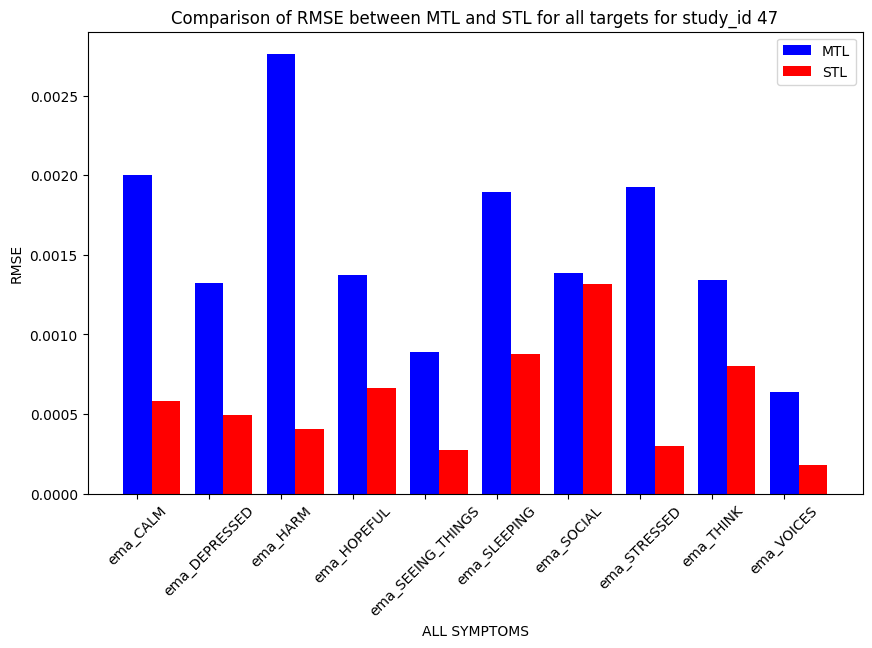
\includegraphics[width=0.5\linewidth]{RMSE_ALL_AUTO_47.png}
    \caption{RMSE FOR STL AND MTL\_ALL FOR STUDY ID 47}
    \label{RMSE_ALL_47}
\end{figure}

\begin{figure}[H]
    \centering
    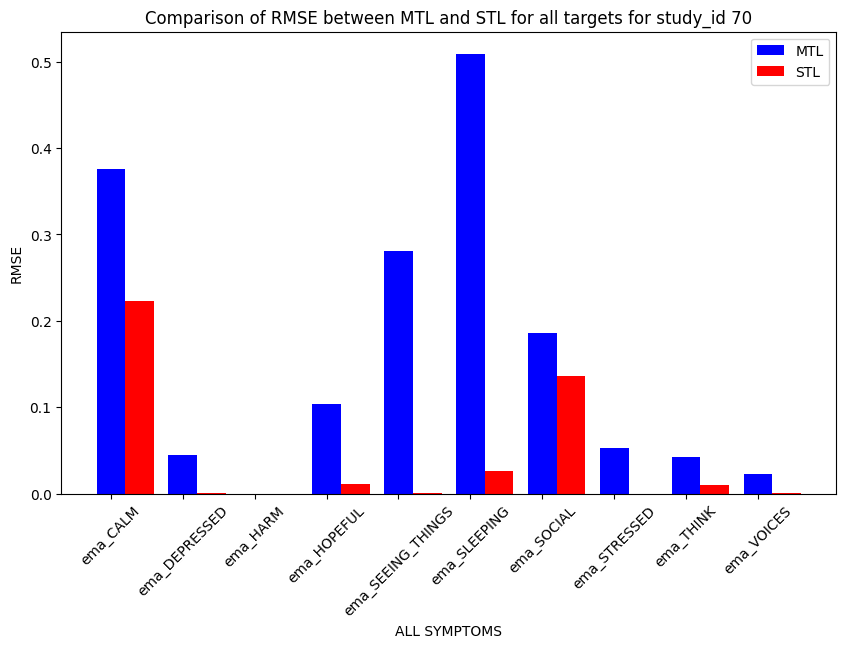
\includegraphics[width=0.5\linewidth]{RMSE_ALL_AUTO_70.png}
    \caption{RMSE FOR STL AND MTL\_ALL FOR STUDY ID 70}
    \label{RMSE_ALL_70}
\end{figure}

Based on the results presented in Figures \ref{RMSE_ALL_47} and \ref{RMSE_ALL_70}, it is evident that Single Task Learning (STL) consistently outperforms Multitask Learning (MTL) across both studies, with Study\_id 47 comprising 408 entries and Study\_id 70 containing 22 entries. The consistently higher RMSE values observed in MTL highlight the potential challenges inherent in multitasking learning, likely due to inadequate or insufficiently distinct shared features for modeling as opposed to the amount to features examined by \citet{tseng2020using}.The smaller dataset size, particularly in Study\_id 70, exacerbates this issue, as MTL depends on sufficient data to effectively learn shared representations across tasks. With limited data, MTL's ability to identify meaningful shared features diminishes, making it more difficult to model individual tasks accurately. This data scarcity can lead to suboptimal shared representations, failing to capture the critical task-specific nuances and resulting in poorer overall performance compared to STL.The statistical significance of these findings is underscored by the p-value of 0.008, indicating a highly significant difference in performance between STL and MTL. This p-value confirms that the observed performance advantage of STL over MTL is not due to random chance, further validating the superiority of task-specific learning models, especially in scenarios with smaller datasets where MTL's shared feature approach is particularly challenged. 

The overall comparative analysis of MTL and STL for all methodologies except the personalized indicates that MTL generally exhibits superior performance than STL, especially when hyperparameters are fine-tuned. This advantage stems from MTL’s ability to leverage inter-task correlations, enhancing its predictive accuracy.




\section{Comparison Against Other Studies}
This study presents a novel approach in comparing single-task learning (STL) and multitask learning (MTL) using a consistent algorithmic framework, specifically LassoCV for STL and its variant MultiTaskLassoCV for MTL. In contrast, \citet{tseng2020using} explored a broader range of algorithms to evaluate both STL and MTL, highlighting that while MTL generally outperformed STL in both generalized and personalized models, only the difference in personalized performance was statistically significant. This divergence underscores the value of comparing STL and MTL within a unified model framework, as seen in the current study, which helps provide a clearer evaluation of model performance by using common evaluation criteria.

Another critical distinction between the studies is the difference in dataset size and feature complexity. While \citet{tseng2020using} utilized 4,157 original features in their analysis, this study examined only 155 features. This stark difference in feature space directly influences the models' capability to capture complex relationships within the data. The impact of this is particularly evident when comparing personalized MTL and STL models, where a higher feature count allows for more nuanced and detailed personalization. The smaller feature set in this study likely constrained the model's ability to fully leverage the personalized advantages of MTL, providing a compelling point of contrast against the findings of \citet{tseng2020using}.

This study’s approach of using the same base algorithm with STL and MTL variants contributes to the literature by providing insights into the performance of models under uniform evaluation conditions, thus avoiding the confounding effects of algorithmic diversity seen in previous studies. This methodological consistency facilitates a more precise understanding of the inherent strengths and limitations of STL and MTL approaches when applied to similar tasks.


\section{Limitations and Scope for Improvement}
\subsection{Limitations}

A primary limitation of this study arises from the dataset size and quality. The relatively small dataset used in this study, coupled with the substantial amount of missing data, poses challenges in achieving robust and personalized results. The limited sample size restricts the statistical power of the findings, and missing data can introduce biases or lead to inaccurate conclusions, especially in personalized models where data sparsity can significantly affect individual predictions.


The computational complexity of the MultiTaskLassoCV model presents another substantial challenge, particularly in the context of personalized modeling with hyperparameter tuning. This approach requires considerable computational resources and extended processing time, especially when handling large-scale or high-dimensional datasets. These demands can become a bottleneck in the model training and optimization process, limiting the scalability and practical applicability of this approach to larger or more complex datasets. Additionally, the increased complexity associated with hyperparameter tuning in MTL can result in suboptimal model performance if not meticulously managed, further complicating the balance between model complexity and computational feasibility.



Another significant limitation is the selection of LassoCV as the model for both STL and MTL comparisons. While LassoCV excels at feature selection and regression through the integration of regularization with cross-validation, it is not specifically tailored for sequential data or temporal machine learning tasks. The application of LassoCV to a time-series dataset limits its effectiveness, as it lacks mechanisms to capture temporal dependencies inherent in sequential data. Models such as Recurrent Neural Networks (RNNs) or Temporal Convolutional Networks (TCNs), which are designed to handle the temporal nature of data, could potentially offer superior predictive performance and interpretability by leveraging these time-dependent relationships.



\subsection{Scope for Improvement}

To enhance the effectiveness of the approach, future research could explore the integration of models specifically designed for time-series analysis, such as Recurrent Neural Network (RNN) or Temporal Convolutional Networks (TCNs). These models can better capture temporal dependencies and might improve the accuracy and interpretability of predictions, particularly for datasets with sequential characteristics. Moreover, expanding the dataset size and improving data quality could help improve model performance and the reliability of results.

To mitigate the computational complexity associated with MultitaskLassoCV, alternative approaches such as dimensionality reduction techniques (e.g., Principal Component Analysis, PCA) could be employed before model training. Additionally, leveraging parallel processing or cloud computing resources might help in managing the computational demands, allowing for more efficient model training and evaluation.



\def\baselinestretch{1.44}

%%% ----------------------------------------------------------------------


   
\smallskip
%%% ----------------------------------------------------------------------
\goodbreak








\def\baselinestretch{1.66}
\medskip

%%% ----------------------------------------------------------------------
 
%\include{Ch5}
%\include{Ch6} 
% ......
\include{EvaluationAndDiscussion}
% ------------------------------------------------------------------------
% -*-TeX-*- -*-Hard-*- Smart Wrapping
% ------------------------------------------------------------------------
\def\baselinestretch{1}

\chapter{Conclusion}

\def\baselinestretch{1.66}

%%% ----------------------------------------------------------------------


%\bigskip

%%% ----------------------------------------------------------------------
\goodbreak
\section{Conclusion}
The comparison between Single Task Learning (STL) using LassoCV and Multi-Task Learning (MTL) using MultiTaskLassoCV reveals significant performance differences in predicting mental health symptoms among schizophrenia patients.  MTL generally achieves lower Root Mean Square Error (RMSE) values compared to STL especially with hyperparameter tuning of the alpha, demonstrating better predictive accuracy across various symptoms. Notably, MTL shows significant improvements over STL in symptoms with ema\_SEEING-THINGS having the lowest RMSE value. MTL's lower RMSE suggests it predicts variations in patients' levels of hallucinations more accurately.


Additionally, it is important to note that both LassoCV and MultitasklassoCV can be effectively utilized in a generalized approach. The findings in this study underscore the statistical significance of the generalized modeling approach, which contrasts with the conclusions drawn by \citet{tseng2020using}. This discrepancy may be attributed to the use of a single model incorporating both single and multitask learning variants, suggesting that the multitask learning variant of a single-task learning offers a more robust framework for identifying and predicting similar symptoms in schizophrenia. While LassoCV remains a valuable tool for single-task predictions, the enhanced performance of MultitasklassoCV indicates its potential for more comprehensive models that address the complexity of schizophrenia symptoms, whether in a generalized or personalized context.

In conclusion, these findings align with the research hypotheses, demonstrating that multitask learning has substantial potential to enhance the accuracy and efficacy of mental health predictions in schizophrenia. By utilizing this approach, clinicians can improve the overall quality of decision-making, leading to more effective and evidence-based treatment strategies for schizophrenia patients. This research highlights the critical role of advanced machine learning techniques in refining mental health care and underscores the potential of multitask learning to support generalized clinical decisions that benefit a broader patient population.

%%% ----------------------------------------------------------------------
\goodbreak
\section{Suggestion for Further Work}
To further advance this research, several promising avenues could be pursued to deepen the understanding and broaden the application of multitask learning in predicting mental health outcomes for schizophrenia patients. First, expanding the study to encompass a larger, more diverse patient population would enhance the generalizability and robustness of findings, validating the effectiveness of LassoCV and MultitaskLassoCV in personalized mental health prediction. By focusing on individualized symptom patterns and responses to treatment, future research could contribute to the development of precision medicine approaches in mental health care. This expansion would also help to capture a wider range of clinical presentations and demographic variations, offering a more comprehensive evaluation of these models in real-world settings.

Additionally, incorporating more advanced and sophisticated machine learning models, such as deep learning techniques, could further improve predictive accuracy and capture more complex patterns in the data.


Moreover, investigating the use of MulitaskLassoCV for multitask learning in other mental health conditions could help to determine whether the observed benefits extend beyond schizophrenia, potentially offering broader implications for mental health prediction and treatment.

Overall, these suggestions for future work aim to build on the promising results of this study, further advancing the application of multitask learning in Schizophrenia prediction and treatment.


 

% ------------------------------------------------------------------------
\setlinespacing{1.44}
\bibliographystyle{agsm} % Use Harvard style 
%\bibliographystyle{apalike}
\bibliography{MyBib} % use your own bib file

%#### Include any appendix below #####
%\appendix
%\include{AppendixA}
%\include{AppendixB}

% =================================================================
\end{document}
% ------------------------------------------------------------------------
